\chapter{Image Processing}
\label{chap:imagebufalgo}
\index{Image Processing|(}
\index{ImageBufAlgo|(}

\IBA is a set of image processing functions that operate on \ImageBuf's.
The functions are declared in the header file
{\cf OpenImageIO/imagebufalgo.h} and are declared in
the {\cf namespace ImageBufAlgo}.


\section{ImageBufAlgo common principles}
\label{sec:iba:intro}

This section explains the general rules common to all \ImageBufAlgo
functions. Only exceptions to these rules will be explained in the
subsequent listings of all the individual \IBA functions.


\subsubsection*{Return values and error messages}

Most \IBA functions that produce image data come in two forms:

\begin{enumerate}
\item Return an \ImageBuf.

The return value is a new \ImageBuf containing the result image. In this
case, an entirely new image will be created to hold the result. In case of
error, the result image returned can have any error conditions checked with
{\cf has_error()} and {\cf geterror()}.

\begin{code}
    // Method 1: Return an image result
    ImageBuf fg ("fg.exr"), bg ("bg.exr");
    ImageBuf dst = ImageBufAlgo::over (fg, bg);
    if (dst.has_error())
        std::cout << "error: " << dst.geterror() << "\n";
\end{code}


\item Pass a destination \ImageBuf reference as the first parameter.

The function is passed a \emph{destination} \ImageBuf where the results will
be stored, and the return value is a {\cf bool} that is {\cf true} if the
function succeeds or {\cf false} if the function fails. Upon failure, the
destination \ImageBuf (the one that is being altered) will have an error
message set.

\begin{code}
    // Method 2: Write into an existing image
    ImageBuf fg ("fg.exr"), bg ("bg.exr");
    ImageBuf dst;   // will be the output image
    bool ok = ImageBufAlgo::over (dst, fg, bg);
    if (! ok)
        std::cout << "error: " << dst.geterror() << "\n";
\end{code}

\end{enumerate}

The first option (return an \ImageBuf directly) is a more compact and
intuitive notation that is natural for most simple uses. But the second
option (pass an {\cf ImageBuf\&} referring to an existing destination)
offers additional flexibility, including more careful control over
allocations, the ability to partially overwrite regions of an existing
image, and the ability for the destination image to also be one of the input
images (for example, add(A,A,B) adds B into existing image A, with no third
image allocated at all).

For a small minority of \IBA functions, there are only input images, and
no image outputs (e.g., {\cf isMonochrome()}).  In such cases, the error
message should be retrieved from the first input image.

\subsubsection*{Region of interest}

Most \IBA functions take an optional \ROI parameter that restricts the
operation to a range in x, y, z, and channels. The default-constructed ROI
(also known as {\cf ROI::All()}) means no region restriction.

For \IBA functions that write into a destination \ImageBuf parameter and it
is already initialized (i.e. allocated with a particular size and data
type), the operation will be performed on the pixels in the destination that
overlap the \ROI, leaving pixels in the destination which are outside the
\ROI unaltered.

For \IBA functions that return an \ImageBuf directly, or if their {\cf dst}
parameter is an uninitialized \ImageBuf, the \ROI (if set) determines the
size of the result image. If the ROI is the default {\cf All}, the result
image size will be the union of the pixel data windows of the input images
and have a data type determind by the data types of the input images.

Most \IBA functions also respect the {\cf chbegin} and {\cf chend}
members of the \ROI, thus restricting the channel range on which the
operation is performed.  The default \ROI constructor sets up the \ROI
to specify that the operation should be performed on all channels of
the input image(s).

\subsection*{Constant and per-channel values}

Many ImageBufAlgo functions take per-channel constant-valued arguments
(for example, a fill color). These parameters are passed as
{\cf cspan<float>}. These are generally expected to have length equal to the
number of channels. But you may also pass a single float which will be
used as the value for all channels. (More generally, what is happening
is that the last value supplied is replicated for any missing channel.)

Some \ImageBufAlgo functions have parameters of type {\cf Image_or_Const},
which may take either an \ImageBuf reference, or a per-channel constant,
or a single constant to be used for all channels.

\subsubsection*{Multithreading}

All \IBA functions take an optional {\cf nthreads} parameter that
signifies the maximum number of threads to use to parallelize the
operation.  The default value for {\cf nthreads} is 0, which signifies
that the number of thread should be the OIIO global default set by {\cf
  OIIO::attribute()} (see Section~\ref{sec:attribute:threads}), which
itself defaults to be the detected level of hardware concurrency (number
of cores available).

Generally you can ignore this parameter (or pass 0), meaning to use all
the cores available in order to perform the computation as quickly as
possible.  The main reason to explicitly pass a different number
(generally 1) is if the application is multithreaded at a high level,
and the thread calling the \IBA function just wants to continue doing
the computation without spawning additional threads, which might tend to
crowd out the other application threads.


\newpage

\section{Pattern generation}
\label{sec:iba:patterns}

For the \IBA functions in this section, there is no ``source'' image.
Therefore, either an initialized {\cf dst} must be supplied (to give a pre-
allocated size and data type of the image), or else it is strictly necessary
to supply an ROI parameter to specify the size of the new image (the data
type in this case will always be {\cf float}). It is an error if one of the
pattern generation \IBA functions is neither supplied a pre-allocated {\cf
dst} nor a non-default \ROI.

\medskip

\apiitem{ImageBuf {\ce zero} (ROI roi, int nthreads=0) \\[1.0ex]
bool {\ce zero} (ImageBuf \&dst, ROI roi=ROI::All(), int nthreads=0)}
\index{ImageBufAlgo!zero} \indexapi{zero}
Create an all-black {\cf float} image of size and channels as described by
the ROI. If {\cf dst} is passed and is alredy initialized, keep its shape and
data type, and just zero out the pixels in the ROI.

\smallskip
\noindent Examples:
\begin{code}
    // Create a new 3-channel, 512x512 float image filled with 0.0 values.
    ImageBuf zero = ImageBufAlgo::zero (ROI(0,512,0,512,0,1,0,3));

    // Zero out an existing buffer, keeping it the same size and data type
    ImageBuf A = ...;
    ...
    ImageBufAlgo::zero (A);

    // Zero out a rectangular region of an existing buffer
    ImageBufAlgo::zero (A, ROI (0, 100, 0, 100));

    // Zero out just the green channel, leave everything else the same
    ROI roi = A.roi ();
    roi.chbegin = 1; // green
    roi.chend = 2;   // one past the end of the channel region
    ImageBufAlgo::zero (A, roi);
\end{code}
\apiend

\apiitem{ImageBuf {\ce fill} (cspan<float> values, ROI roi, int nthreads=0) \\
ImageBuf {\ce fill} (cspan<float> top, cspan<float> bottom, ROI roi, int nthreads=0) \\
ImageBuf {\ce fill} (cspan<float> topleft, cspan<float> topright, \\
  \bigspc\spc cspan<float> bottomleft, cspan<float> bottomright, \\
  \bigspc\spc ROI roi, int nthreads=0) \\[1.0ex]
bool {\ce fill} (ImageBuf \&dst, cspan<float> values, \\
  \bigspc ROI roi=ROI::All(), int nthreads=0) \\
bool {\ce fill} (ImageBuf \&dst, cspan<float> top, cspan<float> bottom, \\
  \bigspc ROI roi=ROI::All(), int nthreads=0) \\
bool {\ce fill} (ImageBuf \&dst, cspan<float> topleft, cspan<float> topright, \\
  \bigspc cspan<float> bottomleft, cspan<float> bottomright, \\
  \bigspc ROI roi=ROI::All(), int nthreads=0)}
\index{ImageBufAlgo!fill} \indexapi{fill}
Fill an image region with given channel values, either returning a new image
or altering the existing dst image within the ROI.  Note that the values
arrays start with channel 0, even if the ROI indicates that a later channel
is the first to be changed.

Three varieties of fill() exist: (a) a single set of channel values that
will apply to the whole ROI, (b) two sets of values that will create a
linearly interpolated gradient from top to bottom of the ROI, (c) four
sets of values that will be bilnearly interpolated across all four
corners of the ROI.

\smallskip
\noindent Examples:
\begin{code}
    // Create a new 640x480 RGB image, with a top-to-bottom gradient
    // from red to pink
    float pink[3] = { 1, 0.7, 0.7 };
    float red[3] = { 1, 0, 0 };
    ImageBuf A = ImageBufAlgo::fill (red, pink, ROI(0, 640, 0, 480, 0, 1, 0, 3));

    // Draw a filled red rectangle overtop existing image A.
    ImageBufAlgo::fill (A, red, ROI(50,100, 75, 175));
\end{code}
\spc 
\includegraphics[width=1.25in]{figures/fill.jpg}  \\
\apiend


\apiitem{ImageBuf {\ce checker} (float width, float height, float depth, \\
\bigspc cspan<float> color1, cspan<float> color2, \\
\bigspc int xoffset, int yoffset, int zoffset, \\
\bigspc ROI roi, int nthreads=0) \\[1.0ex]
bool {\ce checker} (ImageBuf \&dst, float width, float height, float depth, \\
\bigspc cspan<float> color1, cspan<float> color2, \\
\bigspc int xoffset=0, int yoffset=0, int zoffset=0, \\
\bigspc ROI roi=ROI::All(), int nthreads=0)}
\index{ImageBufAlgo!checker} \indexapi{checker}
Create a new image, or set the pixels in the destination image within the
ROI, to a checkerboard pattern with origin given by the {\cf offset} values,
checker size given by the {\cf width, height, depth} values, and  alternting
between {\cf color1[]} and {\cf color2[]}.  The colors must point to arrays
long enough to contain values for all channels in the image.

\smallskip
\noindent Examples:
\begin{code}
    // Create a new 640x480 RGB image, fill it with a two-toned gray
    // checkerboard, the checkers being 64x64 pixels each.
    ImageBuf A (ImageSpec(640, 480, 3, TypeDesc::FLOAT);
    float dark[3] = { 0.1, 0.1, 0.1 };
    float light[3] = { 0.4, 0.4, 0.4 };
    ImageBufAlgo::checker (A, 64, 64, 1, dark, light, 0, 0, 0);
\end{code}
\spc 
\includegraphics[width=1.25in]{figures/checker.jpg}  \\
\apiend


\apiitem{ImageBuf {\ce noise} (string_view noisetype, float A = 0.0f, float B = 0.1f,\\
\bigspc\spc  bool mono = false, int seed = 0, ROI roi=ROI::All(), int nthreads=0) \\[1.0ex]
bool {\ce noise} (ImageBuf \&dst, string_view noisetype, \\
\bigspc\spc float A = 0.0f, float B = 0.1f, bool mono = false, \\
\bigspc\spc int seed = 0, ROI roi=ROI::All(), int nthreads=0)}
\indexapi{noise}

Return an image of pseudorandom noise, or add pseudorandom noise
to the specified region of existing region {\cf dst}.

For noise type \qkw{uniform}, the noise is uniformly distributed on the
range {\cf [A,B)}. For noise \qkw{gaussian}, the noise will have a normal
distribution with mean A and standard deviation B. For noise \qkw{salt}, the
value A will be stored in a random set of pixels whose proportion (of the
overall image) is B. For all noise types, choosing different {\cf seed}
values will result in a different pattern. If the {\cf mono} flag is {\cf
true}, a single noise value will be applied to all channels specified by
{\cf roi}, but if {\cf mono} is {\cf false}, a separate noise value will be
computed for each channel in the region.

\smallskip
\noindent Examples:
\begin{code}
    // Create a new 256x256 field of grayscale uniformly distributed noise on [0,1)
    ImageBuf A = ImageBufAlgo::noise ("uniform", 0.0f /*min*/, 1.0f /*max*/,
                         true /*mono*/, 1 /*seed*/, ROI(0,256,0,256,0,1,0,3));

    // Add color Gaussian noise to an existing image
    ImageBuf B ("tahoe.jpg");
    ImageBufAlgo::noise (B, "gaussian", 0.0f /*mean*/, 0.1f /*stddev*/,
                         false /*mono*/, 1 /*seed*/);

    // Use salt and pepper noise to make occasional random dropouts
    ImageBuf C ("tahoe.jpg");
    ImageBufAlgo::noise (C, "salt", 0.0f /*value*/, 0.01f /*portion*/,
                         true /*mono*/, 1 /*seed*/);
\end{code}

\noindent
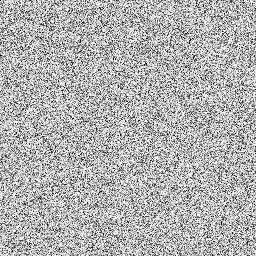
\includegraphics[width=1.25in]{figures/unifnoise1.jpg}
\spc 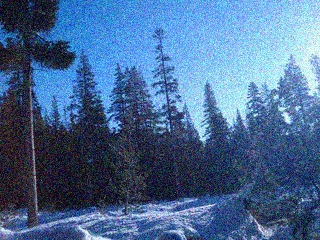
\includegraphics[width=1.65in]{figures/tahoe-gauss.jpg} 
\spc 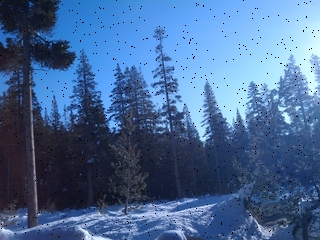
\includegraphics[width=1.65in]{figures/tahoe-pepper.jpg}

\apiend


\apiitem{bool {\ce render_point} (ImageBuf \&dst, int x, int y, cspan<float> color, \\
  \bigspc\spc\spc ROI roi=ROI.All(), int nthreads=0)}
\index{ImageBufAlgo!render_point} \indexapi{render_point}
Render a point into the destination image,  doing an ``over'' of color (if
it includes an alpha channel). The {\cf color} value should have at least as
many entires as the ROI (which will default to being the entirety of
{\cf dst}). No pixels or channels outside the ROI will be modified.

\smallskip
\noindent Examples:
\begin{code}
    ImageBuf A (ImageSpec (640, 480, 4, TypeDesc::FLOAT));
    float red[4] = { 1, 0, 0, 1 };
    ImageBufAlgo::render_point (A, 50, 100, red);
\end{code}
\apiend


\apiitem{bool {\ce render_line} (ImageBuf \&dst, int x1, int y1, int x2, int y2, \\
  \bigspc\spc\spc cspan<float> color, bool skip_first_point=false,\\
  \bigspc\spc\spc ROI roi=ROI.All(), int nthreads=0)}
\index{ImageBufAlgo!render_line} \indexapi{render_line}
Render a line from pixel $(x_1,y_1)$ to $(x_2,y_2)$ into {\cf dst}, doing an
``over'' of the color (if it includes an alpha channel) onto the existing
data in {\cf dst}. The {\cf color} should include as many values as {\cf
roi.chend-1}. The ROI can be used to limit the pixel area or channels that
are modified, and default to the entirety of {\cf dst}. If {\cf skip_first_point}
is {\cf true}, the first point {\cf (x1, y1)} will not be drawn (this can
be helpful when drawing poly-lines, to avoid double-rendering of the
vertex positions).

\smallskip
\noindent Examples:
\begin{code}
    ImageBuf A (ImageSpec (640, 480, 4, TypeDesc::FLOAT));
    float red[4] = { 1, 0, 0, 1 };
    ImageBufAlgo::render_line (A, 10, 60, 250, 20, red);
    ImageBufAlgo::render_line (A, 250, 20, 100, 190, red, true);
\end{code}

\spc 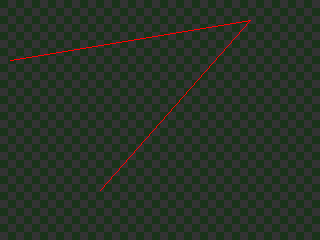
\includegraphics[width=1.65in]{figures/lines.png}  \\
\apiend


\apiitem{bool {\ce render_box} (ImageBuf \&dst, int x1, int y1, int x2, int y2, \\
  \bigspc\spc\spc cspan<float> color, bool fill=false, \\
  \bigspc\spc\spc roi=ROI.All(), int nthreads=0)}
\index{ImageBufAlgo!render_box} \indexapi{render_box}

Render a filled or unfilled box with corners at pixels $(x_1,y_1)$ and
$(x_2,y_2)$ into {\cf dst}, doing an ``over'' of the color (if it includes
an alpha channel) onto the existing data in {\cf dst}. The {\cf color} must
include as many values as {\cf roi.chend-1}. The ROI can be used to limit
the pixel area or channels that are modified, and default to the entirety of
{\cf dst}. If {\cf fill} is {\cf true}, the box will be completely filled in,
otherwise only its outlien will be drawn.

\smallskip
\noindent Examples:
\begin{code}
    ImageBuf A (ImageSpec (640, 480, 4, TypeDesc::FLOAT));
    float cyan[4] = { 1, 0, 0, 1 };
    ImageBufAlgo::render_box (A, 150, 100, 240, 180, cyan);
    float yellow_transparent[4] = { 0.5, 0.5, 0, 0.5 };
    ImageBufAlgo::render_box (A, 100, 50, 180, 140, yellow_transparent, true);
\end{code}

\spc 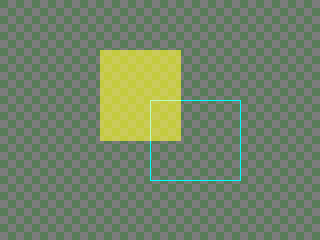
\includegraphics[width=1.65in]{figures/box.png}  \\
\apiend


\apiitem{bool {\ce render_text} (ImageBuf \&dst, int x, int y, string_view text,\\
  \bigspc\spc\spc int fontsize=16, string_view fontname="", \\
  \bigspc\spc\spc  cspan<float> textcolor = 1.0,\\
  \bigspc\spc\spc  TextAlignX alignx = TextAlignX::Left, \\
  \bigspc\spc\spc  TextAlignY aligny = TextAlignX::BaseLine, \\
  \bigspc\spc\spc  int shadow = 0, ROI roi = ROI::All(), int nthreads =0) \\[1.5ex]
  enum class TextAlignX \{ Left, Right, Center \}; \\
  enum class TextAlignY \{ Baseline, Top, Bottom, Center \}; \\[1.0ex]
}
\index{ImageBufAlgo!render_text} \indexapi{render_text}

Render a text string (encoded as UTF-8) into image {\cf dst}. If the {\cf dst} image
is not yet initiailzed, it will be initialized to be a black background
exactly large enought to contain the rasterized text.  If {\cf dst} is already
initialized, the text will be rendered into the existing image by
essentially doing an ``over'' of the character into the existing pixel
data.

The font is given by {\cf fontname} (if not a full pathname to a font file, it
will search for a matching font, defaulting to some reasonable system
font if not supplied at all), and with a nominal height of {\cf fontsize} (in
pixels).

The position is given by coordinates ({\cf x,y}), with the default behavior
to align the left edge of the character baseline to ({\cf x,y}). Optionally,
{\cf alignx} and {\cf aligny} can override the alignment behavior, with horizontal
alignment choices of {\cf Left}, {\cf Right}, and {\cf Center}, and vertical alignment
choices of {\cf Baseline}, {\cf Top}, {\cf Bottom}, or {\cf Center}.

The characters will be drawn in opaque white (1.0,1.0,...) in all channels,
unless {\cf textcolor} is supplied. If {\cf shadow} is nonzero, a ``drop shadow'' of
that radius will be used to make the text look more clear by dilating the
alpha channel of the composite (makes a black halo around the characters).

\smallskip
\noindent Examples:
\begin{code}
    ImageBufAlgo::render_text (ImgA, 50, 100, "Hello, world");

    float red[] = { 1, 0, 0, 1 };
    ImageBufAlgo::render_text (ImgA, 100, 200, "Go Big Red!",
                               60, "Arial Bold", red);

    float white[] = { 1, 1, 1, 1 };
    ImageBufAlgo::render_text (ImgB, 320, 240, "Centered",
                               60, "Arial Bold", white,
                               TextAlignX::Center, TextAlignY::Center);

\end{code}
\spc 
\includegraphics[width=2.5in]{figures/text.jpg}
\spc 
\includegraphics[width=2.5in]{figures/textcentered.jpg} \\
\apiend


\apiitem{ROI {\ce text_size} (string_view text, int fontsize=16,
string_view fontname="")}
\index{ImageBufAlgo!text_size} \indexapi{text_size}

The helper function {\cf text_size()} merely computes the dimensions of the
text, returning it as an {\cf ROI}  relative to the left side of the
baseline of the first character. Only the $x$ and $y$ dimensions of the ROI
will be used. The $x$ dimension runs from left to right, and $y$ runs from
top to bottom (image coordinates). For a failure (such as an invalid
font name), the ROI will return {\cf false} if you call its {\cf defined()}
method.

\begin{code}
    // Render text centered in the image, using text_size to find out
    // the size we will need and adjusting the coordinates.
    ImageBuf A (ImageSpec (640, 480, 4, TypeDesc::FLOAT));
    ROI Aroi = A.roi();
    ROI size = ImageBufAlgo::text_size ("Centered", 48, "Courier New");
    if (size.defined()) {
        int x = Aroi.xbegin + Aroi.width()/2  - (size.xbegin + size.width()/2);
        int y = Aroi.ybegin + Aroi.height()/2 - (size.ybegin + size.height()/2);
        ImageBufAlgo::render_text (A, x, y, "Centered", 48, "Courier New");
    }
\end{code}
%\spc 
\includegraphics[width=2.0in]{figures/textcentered.jpg} \\
\apiend



\newpage

\section{Image transformations and data movement}
\label{sec:iba:transforms}

\apiitem{ImageBuf {\ce channels} (const ImageBuf \&src, int nchannels, \\
        \bigspc  cspan<int> channelorder,  cspan<float> channelvalues=\{\}, \\
        \bigspc  cspan<std::string> newchannelnames=\{\}, \\
        \bigspc  bool shuffle_channel_names=false, int nthreads=0) \\[1.0ex]
bool {\ce channels} (ImageBuf \&dst, const ImageBuf \&src, int nchannels, \\
        \bigspc  cspan<int> channelorder,  cspan<float> channelvalues=\{\}, \\
        \bigspc  cspan<std::string> newchannelnames=\{\}, \\
        \bigspc  bool shuffle_channel_names=false, int nthreads=0)}
\index{ImageBufAlgo!channels} \indexapi{channels} \label{sec:iba:channels}

Generic channel shuffling: return (or store in {\cf dst}) a copy of
{\cf src}, but with channels in the order specified by
{\cf channelorder[0..nchannels-1]}. For any channel in which
{\cf channelorder[i]} $< 0$, it will just make {\cf dst} channel {\cf i} be
a constant value set to {\cf channelvalues[i]} (if {\cf channelvalues} is
not empty) or {\cf 0.0} (if {\cf channelvalues} is empty). In-place
operation is allowed (i.e., dst and src the same image, but an extra copy
will occur).

If {\cf channelorder} is empty, it will be interpreted as
{\cf \{0, 1, ..., nchannels-1\}}, meaning that it's only renaming channels,
not reordering them.

If {\cf newchannelnames} is not empty, it points to an array of new channel
names.  Channels for which {\cf newchannelnames[i]} is the empty string (or
all channels, if {\cf newchannelnames} is empty) will be named as follows:
If {\cf shuffle_channel_names} is {\cf false}, the resulting dst image will have
default channel names in the usual order (\qkw{R}, \qkw{G}, etc.), but if
{\cf shuffle_channel_names} is {\cf true}, the names will be taken from the
corresponding channels of the source image -- be careful with this,
shuffling both channel ordering and their names could result in no
semantic change at all, if you catch the drift.

\smallskip
\noindent Examples:
\begin{code}
    // Copy the first 3 channels of an RGBA, drop the alpha
    ImageBuf RGBA (...);   // assume it's initialized, 4 chans
    ImageBuf RGB = ImageBufAlgo::channels (RGBA, 3, {} /*default ordering*/);

    // Copy just the alpha channel, making a 1-channel image
    ImageBuf Alpha = ImageBufAlgo::channels (RGBA, 1, 3 /*alpha_channel*/);

    // Swap the R and B channels into an existing image
    ImageBuf BRGA;
    int channelorder[] = { 2 /*B*/, 1 /*G*/, 0 /*R*/, 3 /*A*/ };
    ImageBufAlgo::channels (BRGA, RGBA, 4, channelorder);

    // Add an alpha channel with value 1.0 everywhere to an RGB image,
    // keep the other channels with their old ordering, values, and
    // names.
    int channelorder[] = { 0, 1, 2, -1 /*use a float value*/ };
    float channelvalues[] = { 0 /*ignore*/, 0 /*ignore*/, 0 /*ignore*/, 1.0 };
    std::string channelnames[] = { "", "", "", "A" };
    ImageBuf RGBA = ImageBufAlgo::channels (RGB, 4, channelorder,
                                            channelvalues, channelnames);
\end{code}
\apiend

\apiitem{ImageBuf {\ce channel_append} (const ImageBuf \&A, const ImageBuf \&B, \\
        \bigspc\bigspc  ROI roi=ROI::All(), int nthreads=0) \\[1.0ex]
bool {\ce channel_append} (ImageBuf \&dst, const ImageBuf \&A, const ImageBuf \&B, \\
        \bigspc\bigspc  ROI roi=ROI::All(), int nthreads=0)}
\index{ImageBufAlgo!channel_append} \indexapi{channel_append}

Append the channels of {\cf A} and {\cf B} together into {\cf dst} over
the region of interest.  If the region passed is uninitialized (the
default), it will be interpreted as being the union of the pixel windows
of {\cf A} and {\cf B} (and all channels of both images).  If {\cf dst}
is not already initialized, it will be resized to be big enough for the
region.

\smallskip
\noindent Examples:
\begin{code}
    ImageBuf RGBA (...);   // assume initialized, 4 channels
    ImageBuf Z (...);      // assume initialized, 1 channel
    ImageBuf RGBAZ = ImageBufAlgo::channel_append (RGBA, Z);
\end{code}
\apiend


\apiitem{ImageBuf {\ce copy} (const ImageBuf \&src, TypeDesc convert=TypeUnknown, \\
        \bigspc  ROI roi=\{\}, int nthreads=0) \\[1.0ex]
bool {\ce copy} (ImageBuf \&dst, const ImageBuf \&src, TypeDesc convert=TypeUnknown, \\
        \bigspc ROI roi=\{\}, int nthreads=0)}
\index{ImageBufAlgo!copy} \indexapi{copy}

Return (or copy into {\cf dst} at the corresponding locations) the specified
region of pixels of {\cf src}.  If {\cf dst} is not already initialized, it
will be set to the same size as {\cf roi} (by default all of {\cf src},
optionally with the pixel type overridden by {\cf convert} (if it is not
{\cf UNKNOWN}).

\smallskip
\noindent Examples:
\begin{code}
    // Set B to be A, but converted to float
    ImageBuf A (...);  // Assume initialized
    ImageBuf B = ImageBufAlgo::copy (A, TypeDesc::FLOAT);
\end{code}
\apiend


\apiitem{ImageBuf {\ce crop} (const ImageBuf \&src,
        ROI roi=\{\}, int nthreads=0) \\[1.0ex]
bool {\ce crop} (ImageBuf \&dst, const ImageBuf \&src,
        ROI roi=\{\}, int nthreads=0)}
\index{ImageBufAlgo!crop} \indexapi{crop}
Reset {\cf dst} to be the specified region of {\cf src}.
Pixels from {\cf src} which are outside {\cf roi} will not be copied, and
new black pixels will be added for regions of {\cf roi} which were outside
the data window of {\cf src}.

Note that the {\cf crop} operation does not actually move the pixels on the
image plane or adjust the full/display window; it merely restricts which
pixels are copied from {\cf src} to {\cf dst}.  (Note the difference
compared to {\cf cut()}).

\smallskip
\noindent Examples:
\begin{code}
    // Set B to be the upper left 200x100 region of A
    ImageBuf A (...);  // Assume initialized
    ImageBuf B = ImageBufAlgo::crop (A, ROI(0,200,0,100));
\end{code}
\apiend


\apiitem{ImageBuf {\ce cut} (const ImageBuf \&src,
            ROI roi=\{\}, int nthreads=0) \\[1.0ex]
bool {\ce cut} (ImageBuf \&dst, const ImageBuf \&src,
          ROI roi=\{\}, int nthreads=0)}
\index{ImageBufAlgo!cut} \indexapi{cut}
Reset {\cf dst} to be the specified region of {\cf src}, but repositioned at
the image plane origin and with the full/display window set to exactly cover
the new pixel window.  (Note the difference compared to {\cf crop()}).

\smallskip
\noindent Examples:
\begin{code}
    // Set B to be the 100x100 region of A with origin (50,200).
    ImageBuf A (...);  // Assume initialized
    ImageBuf B = ImageBufAlgo::cut (A, ROI(50,250,200,300));
    // Note: B will have origin 0,0, NOT (50,200).
\end{code}
\apiend


\apiitem{bool {\ce paste} (ImageBuf \&dst, int xbegin, int ybegin, int zbegin,
  int chbegin, \\
  \bigspc const ImageBuf \&src, ROI srcroi=ROI::All(), int nthreads=0)}
\index{ImageBufAlgo!paste} \indexapi{paste}
Copy into {\cf dst}, beginning at {\cf (xbegin, ybegin, zbegin)}, the pixels of
{\cf src} described by {\cf srcroi}.  If {\cf srcroi} is {\cf ROI::All()},
the entirety of src will be used.  It will copy into channels
{\cf [chbegin...]}, as many channels as are described by {\cf srcroi}.

\smallskip
\noindent Examples:
\begin{code}
    // Paste small.exr on top of big.exr at offset (100,100)
    ImageBuf Big ("big.exr");
    ImageBuf Small ("small.exr");
    ImageBufAlgo::paste (Big, 100, 100, 0, 0, Small);
\end{code}
\apiend


\apiitem{ImageBuf {\ce rotate90} (const ImageBuf \&src,
          ROI roi=\{\}, int nthreads=0) \\
ImageBuf {\ce rotate180} (const ImageBuf \&src,
          ROI roi=\{\}, int nthreads=0) \\
ImageBuf {\ce rotate270} (const ImageBuf \&src,
          ROI roi=\{\}, int nthreads=0) \\[1.0ex]
bool {\ce rotate90} (ImageBuf \&dst, const ImageBuf \&src,
        ROI roi=\{\}, int nthreads=0) \\
bool {\ce rotate180} (ImageBuf \&dst, const ImageBuf \&src,
        ROI roi=\{\}, int nthreads=0) \\
bool {\ce rotate270} (ImageBuf \&dst, const ImageBuf \&src,
        ROI roi=\{\}, int nthreads=0) }
\index{ImageBufAlgo!rotate90} \indexapi{rotate90}
\index{ImageBufAlgo!rotate180} \indexapi{rotate180}
\index{ImageBufAlgo!rotate270} \indexapi{rotate270}
Return (or copy into {\cf dst}) a copy of the image pixels of {\cf src},
rotated clockwise by 90, 180, or 270 degrees.

\smallskip
\noindent Examples:
\begin{code}
    ImageBuf A ("grid.jpg");
    ImageBuf R90 = ImageBufAlgo::rotate90 (A);
    ImageBuf R170 = ImageBufAlgo::rotate180 (A);
    ImageBuf R270 = ImageBufAlgo::rotate270 (A);
\end{code}

\noindent \begin{tabular}{cccc}
\includegraphics[width=1.25in]{figures/grid-small.jpg} &
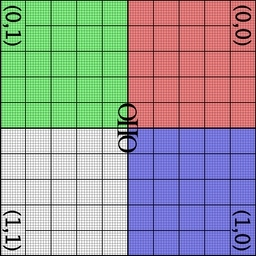
\includegraphics[width=1.25in]{figures/rotate90.jpg} &
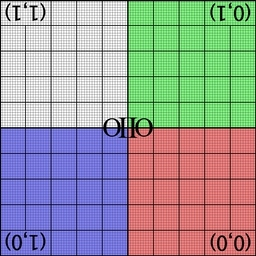
\includegraphics[width=1.25in]{figures/rotate180.jpg} &
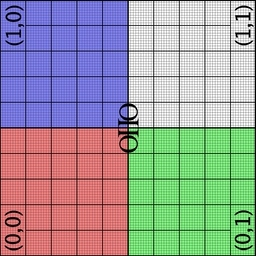
\includegraphics[width=1.25in]{figures/rotate270.jpg} \\
original & rotated 90 & rotated 180 & rotated 270
\end{tabular}
\apiend


\apiitem{ImageBuf {\ce flip} (const ImageBuf \&src, ROI roi=\{\}, int nthreads=0) \\
ImageBuf {\ce flop} (const ImageBuf \&src, ROI roi=\{\}, int nthreads=0) \\
ImageBuf {\ce transpose} (const ImageBuf \&src, ROI roi=\{\}, int nthreads=0) \\[1.0ex]
bool {\ce flip} (ImageBuf \&dst, const ImageBuf \&src, ROI roi=\{\}, int nthreads=0) \\
bool {\ce flop} (ImageBuf \&dst, const ImageBuf \&src, ROI roi=\{\}, int nthreads=0) \\
bool {\ce transpose} (ImageBuf \&dst, const ImageBuf \&src, ROI roi=\{\}, int nthreads=0)
}
\index{ImageBufAlgo!flip} \indexapi{flip}
\index{ImageBufAlgo!flop} \indexapi{flop}
\index{ImageBufAlgo!transpose} \indexapi{transpose}

Return (or copy into {\cf dst}) a subregion of {\cf src}, but with the
scanlines exchanged vertically (flip), or columns exchanged horizontally
(flop), or transposed across the diagonal by swapping rows for columns
(transpose) within the display/full window.

\smallskip
\noindent Examples:
\begin{code}
    ImageBuf A ("grid.jpg");
    ImageBuf B;
    B = ImageBufAlgo::flip (A);
    B = ImageBufAlgo::flop (A);
    B = ImageBufAlgo::transpose (A);
\end{code}

\noindent \begin{tabular}{cccc}
\includegraphics[width=1.25in]{figures/grid-small.jpg} &
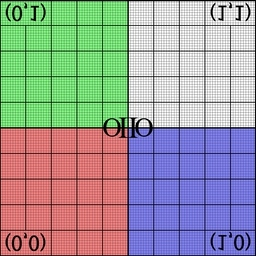
\includegraphics[width=1.25in]{figures/flip.jpg} &
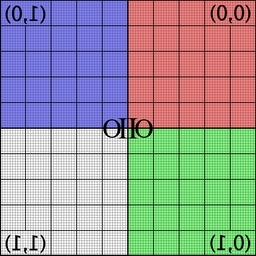
\includegraphics[width=1.25in]{figures/flop.jpg} &
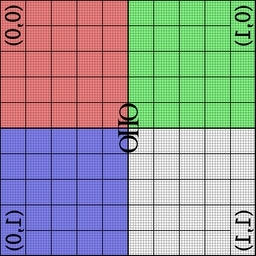
\includegraphics[width=1.25in]{figures/transpose.jpg} \\
original & flip & flip & transpose
\end{tabular}
\apiend


\apiitem{ImageBuf {\ce reorient} (const ImageBuf \&src, int nthreads=0) \\[1.0ex]
bool {\ce reorient} (ImageBuf \&dst, const ImageBuf \&src, int nthreads=0)}
\index{ImageBufAlgo!reorient} \indexapi{reorient}

Return (or store into {\cf dst}) a copy of {\cf src}, but with whatever
seties of rotations, flips, or flops are necessary to transform the pixels
into the configuration suggested by the \qkw{Orientation} metadata of the
image (and the \qkw{Orientation} metadata is then set to 1, ordinary
orientation).

\smallskip
\noindent Examples:
\begin{code}
    ImageBuf A ("tahoe.jpg");
    A = ImageBufAlgo::reorient (A);
\end{code}
\apiend



\apiitem{ImageBuf {\ce circular_shift} (const ImageBuf \&src, \\
        \bigspc int xshift, int yshift, int zshift=0,
        ROI roi=\{\}, int nthreads=0) \\[1.0ex]
bool {\ce circular_shift} (ImageBuf \&dst, const ImageBuf \&src, \\
        \bigspc int xshift, int yshift, int zshift=0,
        ROI roi=\{\}, int nthreads=0)}
\index{ImageBufAlgo!circular_shift} \indexapi{circular_shift}

Copy {\cf src} (or a subregion of {\cf src} to the pixels of {\cf dst},
but circularly shifting by the given amount.  To clarify, the circular
shift of $[0,1,2,3,4,5]$ by $+2$ is $[4,5,0,1,2,3]$.

\smallskip
\noindent Examples:
\begin{code}
    ImageBuf A ("grid.jpg");
    ImageBuf B = ImageBufAlgo::circular_shift (A, 70, 30);
\end{code}
\spc \includegraphics[width=1.25in]{figures/grid-small.jpg} 
~ {\Huge $\rightarrow$} ~
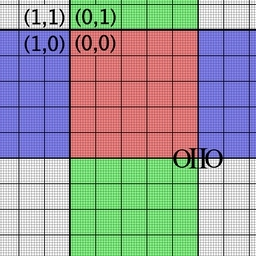
\includegraphics[width=1.25in]{figures/cshift.jpg} \\
\apiend


\apiitem{ImageBuf {\ce rotate} (const ImageBuf \&src, float angle,\\
        \bigspc string_view filtername="", float filtersize=0, \\
        \bigspc bool recompute_roi = false, ROI roi=\{\}, int nthreads=0) \\
ImageBuf {\ce rotate} (const ImageBuf \&src, float angle,\\
        \bigspc Filter2D *filter, \\
        \bigspc bool recompute_roi = false, ROI roi=\{\}, int nthreads=0) \\
ImageBuf {\ce rotate} (const ImageBuf \&src, float angle,\\
        \bigspc float center_x, float center_y, \\
        \bigspc string_view filtername="", float filtersize=0, \\
        \bigspc bool recompute_roi = false, ROI roi=\{\}, int nthreads=0) \\
ImageBuf {\ce rotate} (const ImageBuf \&src, float angle,\\
        \bigspc float center_x, float center_y, Filter2D *filter, \\
        \bigspc bool recompute_roi = false, ROI roi=\{\}, int nthreads=0) \\[1.0ex]
bool {\ce rotate} (ImageBuf \&dst, const ImageBuf \&src, float angle,\\
        \bigspc string_view filtername="", float filtersize=0, \\
        \bigspc bool recompute_roi = false, ROI roi=\{\}, int nthreads=0) \\
bool {\ce rotate} (ImageBuf \&dst, const ImageBuf \&src, float angle,\\
        \bigspc Filter2D *filter, \\
        \bigspc bool recompute_roi = false, ROI roi=\{\}, int nthreads=0) \\
bool {\ce rotate} (ImageBuf \&dst, const ImageBuf \&src, float angle,\\
        \bigspc float center_x, float center_y, \\
        \bigspc string_view filtername="", float filtersize=0, \\
        \bigspc bool recompute_roi = false, ROI roi=\{\}, int nthreads=0) \\
bool {\ce rotate} (ImageBuf \&dst, const ImageBuf \&src, float angle,\\
        \bigspc float center_x, float center_y, Filter2D *filter, \\
        \bigspc bool recompute_roi = false, ROI roi=\{\}, int nthreads=0)}
\index{ImageBufAlgo!rotate} \indexapi{rotate}

Rotate the {\cf src} image by the {\cf angle} (in radians, with positive
angles clockwise). When {\cf center_x} and {\cf center_y} are supplied, they
denote the center of rotation; in their absence, the rotation will be about
the center of the image's display window.

Only the pixels (and channels) of {\cf dst} that are specified by {\cf roi}
will be copied from the rotated {\cf src}; the default {\cf roi} is to alter
all the pixels in {\cf dst}. If {\cf dst} is uninitialized, it will be
resized to be an ImageBuf large enough to hold the rotated image  if
{\cf recompute_roi} is {\cf true}, or will have the same ROI as {\cf src}
if {\cf recompute_roi} is false. It is an
error to pass both an uninitialied {\cf dst} and an undefined {\cf roi}.

The caller may explicitly pass a reconstruction filter, or specify one by
name and size, or if the name is the empty string {\cf rotate()} will choose
a reasonable high-quality default if \NULL is passed.  The filter is used to
weight the {\cf src} pixels falling underneath it for each {\cf dst} pixel;
the filter's size is expressed in pixel units of the {\cf dst} image.

\smallskip
\noindent Examples:
\begin{code}
    ImageBuf Src ("tahoe.exr");
    ImageBuf Dst = ImageBufAlgo::rotate (Src, 45.0);
\end{code}
\spc \includegraphics[width=1.25in]{figures/grid-small.jpg} 
~ {\Huge $\rightarrow$} ~
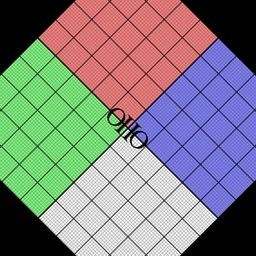
\includegraphics[width=1.25in]{figures/rotate45.jpg} \\
\apiend


\apiitem{ImageBuf {\ce warp} (const ImageBuf \&src, const Imath::M33f \&M, \\
        \bigspc string_view filtername="", float filtersize=0, \\
        \bigspc bool recompute_roi = false, \\
        \bigspc ImageBuf::WrapMode wrap = ImageBuf::WrapDefault, \\
        \bigspc ROI roi=\{\}, int nthreads=0) \\
ImageBuf {\ce warp} (const ImageBuf \&src, const Imath::M33f \&M, \\
        \bigspc Filter2D *filter, bool recompute_roi = false, \\
        \bigspc ImageBuf::WrapMode wrap = ImageBuf::WrapDefault, \\
        \bigspc ROI roi=\{\}, int nthreads=0) \\[1.0ex]
bool {\ce warp} (ImageBuf \&dst, const ImageBuf \&src, const Imath::M33f \&M, \\
        \bigspc string_view filtername="", float filtersize=0, \\
        \bigspc bool recompute_roi = false, \\
        \bigspc ImageBuf::WrapMode wrap = ImageBuf::WrapDefault, \\
        \bigspc ROI roi=\{\}, int nthreads=0) \\
bool {\ce warp} (ImageBuf \&dst, const ImageBuf \&src, const Imath::M33f \&M, \\
        \bigspc Filter2D *filter, bool recompute_roi = false, \\
        \bigspc ImageBuf::WrapMode wrap = ImageBuf::WrapDefault, \\
        \bigspc ROI roi=\{\}, int nthreads=0) }
\index{ImageBufAlgo!warp} \indexapi{warp}

Warp the {\cf src} image using the supplied 3x3 transformation matrix {\cf M}.

Only the pixels (and channels) of {\cf dst} that are specified by {\cf roi}
will be copied from the warped {\cf src}; the default {\cf roi} is to alter
all the pixels in {\cf dst}. If {\cf dst} is uninitialized, it will be
resized to be an \ImageBuf large enough to hold the warped image if
{\cf recompute_roi} is {\cf true}, or will have the same ROI as {\cf src}
if {\cf recompute_roi} is false. It is an
error to pass both an uninitialied {\cf dst} and an undefined {\cf roi}.

The caller may explicitly pass a reconstruction filter, or specify one by
name and size, or if the name is the empty string {\cf resize()} will choose
a reasonable high-quality default if \NULL is passed.  The filter is used to
weight the {\cf src} pixels falling underneath it for each {\cf dst} pixel;
the filter's size is expressed in pixel units of the {\cf dst} image.

\smallskip
\noindent Examples:
\begin{code}
    Imath::M33f M ( 0.7071068, 0.7071068, 0,
                   -0.7071068, 0.7071068, 0,
                   20,        -8.284271,  1);
    ImageBuf Src ("tahoe.exr");
    ImageBuf Dst = ImageBufAlgo::warp (dst, src, M, "lanczos3");
\end{code}
\apiend


\apiitem{ImageBuf {\ce resize} (const ImageBuf \&src, string_view filtername="", \\
        \bigspc  float filtersize=0, ROI roi=\{\}, int nthreads=0) \\
ImageBuf {\ce resize} (const ImageBuf \&src, Filter2D *filter, \\
        \bigspc  ROI roi=\{\}, int nthreads=0) \\[1.0ex]
bool {\ce resize} (ImageBuf \&dst, const ImageBuf \&src, string_view filtername="", \\
        \bigspc  float filtersize=0, ROI roi=\{\}, int nthreads=0) \\
bool {\ce resize} (ImageBuf \&dst, const ImageBuf \&src, Filter2D *filter, \\
        \bigspc  ROI roi=\{\}, int nthreads=0)}
\index{ImageBufAlgo!resize} \indexapi{resize}
Set {\cf dst}, over the region of interest, to be a resized version of the
corresponding portion of {\cf src} (mapping such that the ``full'' image
window of each correspond to each other, regardless of resolution).  If
{\cf dst} is not yet initialized, it will be sized according to {\cf roi}.

The caller may explicitly pass a reconstruction filter, or specify one by
name and size, or if the name is the empty string {\cf resize()} will choose
a reasonable high-quality default if \NULL is passed.  The filter is used to
weight the {\cf src} pixels falling underneath it for each {\cf dst} pixel;
the filter's size is expressed in pixel units of the {\cf dst} image.

\smallskip
\noindent Examples:
\begin{code}
    // Resize the image to 640x480, using the default filter
    ImageBuf Src ("tahoe.exr");
    ROI roi (0, 640, 0, 480, 0, 1, /*chans:*/ 0, Src.nchannels());
    ImageBuf Dst = ImageBufAlgo::resize (Src, "", 0, roi);
\end{code}
\apiend


\apiitem{ImageBuf {\ce resample} (const ImageBuf \&src, \\
        \bigspc bool interpolate = true, ROI roi=\{\}, int nthreads=0) \\[1.0ex]
bool {\ce resample} (ImageBuf \&dst, const ImageBuf \&src, \\
        \bigspc bool interpolate = true, ROI roi=\{\}, int nthreads=0)}
\index{ImageBufAlgo!resample} \indexapi{resample}
Set {\cf dst}, over the region of interest, to be a resized version of the
corresponding portion of {\cf src} (mapping such that the ``full'' image
window of each correspond to each other, regardless of resolution).  If
{\cf dst} is not yet initialized, it will be sized according to {\cf roi}.

Unlike {\cf ImageBufAlgo::resize()}, {\cf resample()} does not take a filter; it
just samples either with a bilinear interpolation (if {\cf interpolate} is
{\cf true}, the default) or uses the single ``closest'' pixel (if
{\cf interpolate} is {\cf false}).  This makes it a lot faster than a proper
{\cf resize()}, though obviously with lower quality (aliasing when
downsizing, pixel replication when upsizing).

For ``deep'' images, this function returns copies the closest source pixel
needed, rather than attempting to interpolate deep pixels (regardless of the
value of {\cf interpolate}).

\smallskip
\noindent Examples:
\begin{code}
    // Resample quickly to 320x240, using the default filter
    ImageBuf Src ("tahoe.exr");
    ROI roi (0, 320, 0, 240, 0, 1, /*chans:*/ 0, Src.nchannels());
    ImageBuf Dst = ImageBufAlgo::resample (Src, false, roi);
\end{code}
\apiend



\section{Image arithmetic}
\label{sec:iba:arith}

\apiitem{ImageBuf {\ce add} (Image_or_Const A, Image_or_Const B, ROI roi=\{\}, int nthreads=0) \\[1.0ex]
bool {\ce add} (ImageBuf \&dst, Image_or_Const A, Image_or_Const B, \\
        \bigspc  ROI roi=\{\}, int nthreads=0)}
\index{ImageBufAlgo!add} \indexapi{add}

Compute per-pixel sum {\cf A + B}, returning the result image or storing
the result into existing image {\cf dst}.

{\cf A} and {\cf B} may each either be an {\cf ImageBuf\&}, or a
{\cf cspan<float>} giving a per-channel constant, or a single constant used
for all channels. (But at least one must be an image.)

\smallskip
\noindent Examples:
\begin{code}
    // Add images A and B, assign to Sum
    ImageBuf A ("a.exr");
    ImageBuf B ("b.exr");
    ImageBuf Sum = ImageBufAlgo::add (Sum, A, B);

    // Add 0.2 to channels 0-2 of A
    ImageBuf A ("a.exr");
    ROI roi = get_roi (A.spec());
    roi.chbegin = 0;  roi.chend = 3;
    ImageBuf Sum = ImageBufAlgo::add (Sum, A, 0.2f, roi);
\end{code}
\apiend



\apiitem{ImageBuf {\ce sub} (Image_or_Const A, Image_or_Const B, ROI roi=\{\}, int nthreads=0) \\[1.0ex]
bool {\ce sub} (ImageBuf \&dst, Image_or_Const A, Image_or_Const B, \\
        \bigspc  ROI roi=\{\}, int nthreads=0)}
\index{ImageBufAlgo!sub} \indexapi{sub}

Compute per-pixel signed difference {\cf A - B}, returning the result image
or storing the result into existing image {\cf dst}.

{\cf A} and {\cf B} may each either be an {\cf ImageBuf\&}, or a
{\cf cspan<float>} giving a per-channel constant, or a single constant used
for all channels. (But at least one must be an image.)

\smallskip
\noindent Examples:
\begin{code}
    ImageBuf A ("a.exr");
    ImageBuf B ("b.exr");
    ImageBuf Diff = ImageBufAlgo::sub (A, B);
\end{code}
\apiend


\apiitem{ImageBuf {\ce absdiff} (Image_or_Const A, Image_or_Const B, ROI roi=\{\}, int nthreads=0) \\[1.0ex]
bool {\ce absdiff} (ImageBuf \&dst, Image_or_Const A, Image_or_Const B, \\
        \bigspc  ROI roi=\{\}, int nthreads=0)}
\index{ImageBufAlgo!absdiff} \indexapi{absdiff}

Compute per-pixel absolute difference {\cf abs(A - B)}, returning the result image
or storing the result into existing image {\cf dst}.

{\cf A} and {\cf B} may each either be an {\cf ImageBuf\&}, or a
{\cf cspan<float>} giving a per-channel constant, or a single constant used
for all channels. (But at least one must be an image.)

\smallskip
\noindent Examples:
\begin{code}
    ImageBuf A ("a.exr");
    ImageBuf B ("b.exr");
    ImageBuf Diff = ImageBufAlgo::absdiff (A, B);
\end{code}
\apiend


\apiitem{ImageBuf {\ce abs} (const ImageBuf \&A, ROI roi=\{\}, int nthreads=0) \\[1.0ex]
bool {\ce abs} (ImageBuf \&dst, const ImageBuf \&A, ROI roi=\{\}, int nthreads=0)}
\index{ImageBufAlgo!abs} \indexapi{abs}

Compute per-pixel absolute value {\cf abs(A)}, returning the result image
or storing the result into existing image {\cf dst}.

\smallskip
\noindent Examples:
\begin{code}
    ImageBuf A ("a.exr");
    ImageBuf Abs = ImageBufAlgo::abs (A);
\end{code}
\apiend



\apiitem{ImageBuf {\ce mul} (Image_or_Const A, Image_or_Const B, ROI roi=\{\}, int nthreads=0) \\[1.0ex]
bool {\ce mul} (ImageBuf \&dst, Image_or_Const A, Image_or_Const B, \\
        \bigspc  ROI roi=\{\}, int nthreads=0)}
\index{ImageBufAlgo!mul} \indexapi{mul}

Compute per-pixel product {\cf A * B}, returning the result image
or storing the result into existing image {\cf dst}.

{\cf A} and {\cf B} may each either be an {\cf ImageBuf\&}, or a
{\cf cspan<float>} giving a per-channel constant, or a single constant used
for all channels. (But at least one must be an image.)

\smallskip
\noindent Examples:
\begin{code}
    ImageBuf A ("a.exr");
    ImageBuf B ("b.exr");
    ImageBuf Product = ImageBufAlgo::mul (Product, A, B);

    // Reduce intensity of A's channels 0-2 by 50%
    ROI roi = get_roi (A.spec());
    roi.chbegin = 0;  roi.chend = 3;
    ImageBufAlgo::mul (A, A, 0.5f, roi);
\end{code}
\apiend


\apiitem{ImageBuf {\ce div} (Image_or_Const A, Image_or_Const B, ROI roi=\{\}, int nthreads=0) \\[1.0ex]
bool {\ce div} (ImageBuf \&dst, Image_or_Const A, Image_or_Const B, \\
        \bigspc  ROI roi=\{\}, int nthreads=0)}
\index{ImageBufAlgo!div} \indexapi{div}

Compute per-pixel division {\cf A / B}, returning the result image
or storing the result into existing image {\cf dst}.
Division by zero is definied to result in zero.

{\cf A} and {\cf B} may each either be an {\cf ImageBuf\&}, or a
{\cf cspan<float>} giving a per-channel constant, or a single constant used
for all channels. (But at least one must be an image.)

\smallskip
\noindent Examples:
\begin{code}
    ImageBuf A ("a.exr");
    ImageBuf B ("b.exr");
    ImageBuf Result = ImageBufAlgo::div (Result, A, B);

    // Reduce intensity of A's channels 0-2 by 50%
    ROI roi = get_roi (A.spec());
    roi.chbegin = 0;  roi.chend = 3;
    ImageBufAlgo::div (A, A, 2.0f, roi);
\end{code}
\apiend


\apiitem{ImageBuf {\ce mad} (Image_or_Const A, Image_or_Const B, \\
        \bigspc  Image_or_Const C, ROI roi=\{\}, int nthreads=0) \\[1.0ex]
bool {\ce mad} (ImageBuf \&dst, Image_or_Const A, Image_or_Const B, \\
        \bigspc  Image_or_Const C, ROI roi=\{\}, int nthreads=0)}
\index{ImageBufAlgo!mad} \indexapi{mad}

Compute per-pixel multiply-and-add, {\cf A * B + C}, returning the result image
or storing the result into existing image {\cf dst}.

{\cf A}, {\cf B}, and {\cf C} may each either be an {\cf ImageBuf\&}, or a
{\cf cspan<float>} giving a per-channel constant, or a single constant used
for all channels. (But at least one must be an image.)

\smallskip
\noindent Examples:
\begin{code}
    ImageBuf A ("a.exr");
    ImageBuf B ("b.exr");
    ImageBuf C ("c.exr");
    ImageBuf Result = ImageBufAlgo::mad (A, B, C);

    // Compute the "inverse" A, which is 1.0-A, as A*(-1) + 1
    // Do this in-place, and only for the first 3 channels (leave any
    // alpha channel, if present, as it is).
    ROI roi = get_roi (A.spec());
    roi.chbegin = 0;  roi.chend = 3;
    ImageBufAlgo::mad (A, A, -1.0, 1.0, roi);
\end{code}
\apiend


\apiitem{ImageBuf {\ce invert} (const ImageBuf \&A, ROI roi=\{\}, int nthreads=0) \\[1.0ex]
bool {\ce invert} (ImageBuf \&dst, const ImageBuf \&A, ROI roi=\{\}, int nthreads=0)}
\index{ImageBufAlgo!invert} \indexapi{invert}

Compute per-pixel inverse, {\cf 1.0 - A}, returning the result image
or storing the result into existing image {\cf dst}.

\smallskip
\noindent Examples:
\begin{code}
    ImageBuf A ("a.exr");
    ImageBuf Inverse = ImageBufAlgo::invert (Inverse, A);

    // In this example, we are careful to deal with alpha in an RGBA image.
    // First we copy A to Inverse, un-premultiply the color values by alpha,
    // invert just the color channels in-place, and then re-premultiply the
    // colors by alpha.
    roi = A.roi();
    roi.chend = 3;      // Restrict roi to only R,G,B
    ImageBuf Inverse = ImageBufAlgo::unpremult (A);
    ImageBufAlgo::invert (Inverse, Inverse, roi);
    ImageBufAlgo::premult (Inverse, Inverse);
\end{code}

%\spc \includegraphics[width=1.5in]{figures/tahoe-small.jpg}
%\raisebox{40pt}{\large $\rightarrow$}
%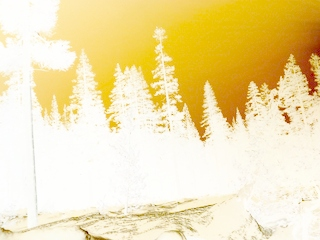
\includegraphics[width=1.5in]{figures/invert.jpg} \\
\apiend


\apiitem{ImageBuf {\ce pow} (const ImageBuf \&A, cspan<float> B, ROI roi=\{\}, int nthreads=0)) \\[1.0ex]
bool {\ce pow} (ImageBuf \&dst, const ImageBuf \&A, cspan<float> B, \\
        \bigspc ROI roi=\{\}, int nthreads=0)}
\index{ImageBufAlgo!pow} \indexapi{pow}

Compute per-pixel power $A^B$, returning the result image
or storing the result into existing image {\cf dst}.

{\cf A} is always an image, and {\cf B} may either be
a {\cf cspan<float>} giving a per-channel constant, or a single constant
used for all channels.

\smallskip
\noindent Examples:
\begin{code}
    // Gamma-correct by 2.2 channels 0-2 of the image, in-place
    ROI roi = get_roi (A.spec());
    roi.chbegin = 0;  roi.chend = 3;
    ImageBufAlgo::pow (A, A, 1.0f/2.2f, roi);
\end{code}
\apiend


\apiitem{ImagBuf {\ce channel_sum} (const ImageBuf \&src, \\
        \bigspc\spc cspan<float> weights=1.0f, ROI roi=\{\}, int nthreads=0) \\[1.0ex]
bool {\ce channel_sum} (ImageBuf \&dst, const ImageBuf \&src, \\
        \bigspc\spc cspan<float> weights=1.0f, ROI roi=\{\}, int nthreads=0)}
\index{ImageBufAlgo!channel_sum} \indexapi{channel_sum}
Converts a multi-channel image into a 1-channel image via a weighted sum
of channels.  For each pixel of {\cf src} within the designated ROI
(defaulting to all of {\cf src}, if not defined), sum the channels
designated by {\cf roi} and store the result in channel 0 of {\cf dst}.
The {\cf weights}, if not supplied, default to 1.0 for each channel.

\smallskip
\noindent Examples:
\begin{code}
    // Compute luminance via a weighted sum of R,G,B
    // (assuming Rec709 primaries and a linear scale)
    float luma_weights[3] = { .2126, .7152, .0722, 0.0 };
    ImageBuf A ("a.exr");
    ImageBuf lum = ImageBufAlgo::channel_sum (A, luma_weights);
\end{code}
\apiend



\apiitem{ImageBuf {\ce color_map} (const ImageBuf \&src, int srcchannel, \\
        \bigspc\spc int nknots, int channels, cspan<float> knots, \\
        \bigspc\spc ROI roi=\{\}, int nthreads=0) \\
ImageBuf {\ce color_map} (const ImageBuf \&src, int srcchannel, \\
        \bigspc\spc string_view mapname, ROI roi=\{\}, int nthreads=0) \\[1.0ex]
bool {\ce color_map} (ImageBuf \&dst, const ImageBuf \&src, int srcchannel, \\
        \bigspc\spc int nknots, int channels, cspan<float> knots, \\
        \bigspc\spc ROI roi=\{\}, int nthreads=0) \\
bool {\ce color_map} (ImageBuf \&dst, const ImageBuf \&src, int srcchannel, \\
        \bigspc\spc string_view mapname, ROI roi=\{\}, int nthreads=0)}
\index{ImageBufAlgo!color_map} \indexapi{color_map}

Return (or copy into {\cf dst}) pixel values determined by looking up a
color map using values of the {\cf src} image, using either the channel
specified by {\cf srcchannel}, or the luminance of {\cf src}'s RGB if {\cf
srcchannel} is -1. This happens for all pixels within the ROI (which
defaults to all of {\cf src}), and if {\cf dst} is not already initialized,
it will be initialized to the ROI and with color channels equal to {\cf channels}.

In the first variant, the values linearly-interpolated color map are
given by {\cf knots[nknots*channels]}.
An input value of 0.0 corresponds to {\cf knots[0..channels-1]}, an input
value of 1.0 corresponds to {\cf knots[(nknots-1)*channels..knots.size()-1]}.

In the second variant, just the name of a color map is specified. Recognized
map names include: \qkw{inferno}, \qkw{viridis}, \qkw{magma}, \qkw{plasma},
all of which are perceptually uniform, strictly increasing in luminance,
look good when converted to grayscale, and work for people with all types of
colorblindness. Also supported are the following color maps that do not have
those desirable qualities (and are this not recommended): \qkw{blue-red},
\qkw{spectrum}, and \qkw{heat}. In all cases, the implied {\cf channels} is
3.

\smallskip
\noindent Examples:
\begin{code}
    // Use luminance of a.exr (assuming Rec709 primaries and a linear
    // scale) and map to a color spectrum:
    ImageBuf A ("a.exr");
    ImageBuf B = ImageBufAlgo::color_map (B, A, -1, "inferno");

    float mymap[] = { 0.25, 0.25, 0.25,  0, 0.5, 0,  1, 0, 0 };
    B = ImageBufAlgo::color_map (A, -1 /* use luminance */,
                                 3 /* num knots */, 3 /* channels */,
                                 mymap);
\end{code}

\noindent \begin{tabular}{ccccc}
\includegraphics[width=0.9in]{figures/tahoe-small.jpg} &
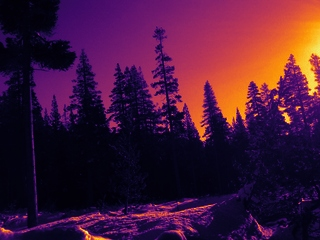
\includegraphics[width=0.9in]{figures/colormap-inferno.jpg} &
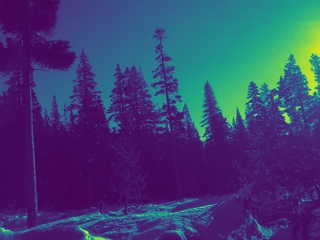
\includegraphics[width=0.9in]{figures/colormap-viridis.jpg} &
\includegraphics[width=0.9in]{figures/colormap-spectrum.jpg} &
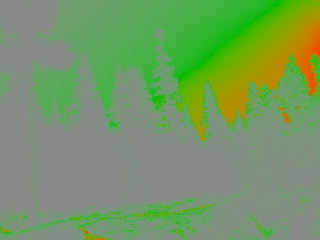
\includegraphics[width=0.9in]{figures/colormap-custom.jpg} \\
original & inferno & viridis & spectrum & custom values \\
\end{tabular}
\apiend



\apiitem{ImageBuf {\ce clamp} (const ImageBuf \&src, \\
  \bigspc cspan<float> min = \{\}, cspan<float> max = \{\}, \\
  \bigspc bool clampalpha01 = false, ROI roi=\{\}, int nthreads=0) \\[1.0ex]
bool {\ce clamp} (ImageBuf \&dst, const ImageBuf \&src, \\
  \bigspc cspan<float> min = \{\}, cspan<float> max = \{\}, \\
  \bigspc bool clampalpha01 = false, ROI roi=\{\}, int nthreads=0)}
\index{ImageBufAlgo!clamp} \indexapi{clamp}

Return (or copy into {\cf dst}) pixels of {\cf src} with pixel values
clamped between the {\cf min} and {\cf max} values. The {\cf min} and
{\cf max} may either be a single float (applied to all channels) or a
per-channel value. If either is empty, no clamping will be performed in
that direction. If {\cf clampalpha01} is {\cf true}, then any alpha
channel is clamped to the 0--1 range (in addition to its otherwise-specified
min/max).

\smallskip
\noindent Examples:
\begin{code}
    // Clamp image buffer A in-place to the [0,1] range for all pixels.
    ImageBufAlgo::clamp (A, A, 0.0f, 1.0f);

    // Just clamp alpha to [0,1] in-place
    ImageBufAlgo::clamp (A, A, -std::numeric_limits<float>::max(),
                         std::numeric_limits<float>::max(), true);

    // Clamp R & G to [0,0.5], leave other channels alone
    std::vector<float> min (A.nchannels(), -std::numeric_limits<float>::max());
    std::vector<float> max (A.nchannels(), std::numeric_limits<float>::max());
    min[0] = 0.0f;  max[0] = 0.5f;
    min[1] = 0.0f;  max[1] = 0.5f;
    ImageBufAlgo::clamp (A, A, &min[0], &max[0], false);
\end{code}
\apiend


\apiitem{ImageBuf {\ce rangecompress} (const ImageBuf \&src, bool useluma = false, \\
        \bigspc\bigspc  ROI roi=\{\}, int nthreads=0) \\
bool {\ce rangecompress} (ImageBuf \&dst, const ImageBuf \&src, bool useluma = false, \\
        \bigspc\bigspc  ROI roi=\{\}, int nthreads=0) \\[1.0ex]
ImageBuf {\ce rangeexpand} (const ImageBuf \&src, bool useluma = false, \\
        \bigspc\bigspc  ROI roi=\{\}, int nthreads=0) \\
bool {\ce rangeexpand} (ImageBuf \&dst, const ImageBuf \&src, bool useluma = false, \\
        \bigspc\bigspc  ROI roi=\{\}, int nthreads=0) }
\index{ImageBufAlgo!rangecompress} \indexapi{rangecompress}
\index{ImageBufAlgo!rangeexpand} \indexapi{rangeexpand}

The {\cf rangecompress()} function returns (or copy into dst) all pixels and
color channels of {\cf src} within region {\cf roi} (defaulting to all the
defined pixels of {\cf dst}), rescaling their range with a logarithmic
transformation. Alpha and z channels are not transformed.

The {\cf rangeexpand()} function performs the inverse transformation
(logarithmic back into linear).

If {\cf useluma} is true, the luma of the first three channels (presumed
to be R, G, and B) are used to compute a single scale factor for all
color channels, rather than scaling all channels individually (which
could result in a big color shift when performing {\cf rangecompress}
and {\cf rangeexpand}).

The purpose of these function is as follows: Some image operations (such
as resizing with a ``good'' filter that contains negative lobes) can have
objectionable artifacts when applied to images with very high-contrast
regions involving extra bright pixels (such as highlights in HDR
captured or rendered images).  By compressing the range pixel values,
then performing the operation, then expanding the range of the result
again, the result can be much more pleasing (even if not exactly
correct).

\smallskip
\noindent Examples:
\begin{code}
    // Resize the image to 640x480, using a Lanczos3 filter, which
    // has negative lobes. To prevent those negative lobes from
    // producing ringing or negative pixel values for HDR data,
    // do range compression, then resize, then re-expand the range.

    // 1. Read the original image
    ImageBuf Src ("tahoeHDR.exr");

    // 2. Range compress to a logarithmic scale
    ImageBuf Compressed = ImageBufAlgo::rangecompress (Src);

    // 3. Now do the resize
    ImageBuf Dst = ImageBufAlgo::resize (Comrpessed, "lanczos3", 6.0,
                                         ROI(0, 640, 0, 480));

    // 4. Expand range to be linear again (operate in-place)
    ImageBufAlgo::rangeexpand (Dst, Dst);
\end{code}
\apiend


\apiitem{ImageBuf {\ce over} (const ImageBuf \&A, const ImageBuf \&B, \\
        \bigspc  ROI roi=\{\}, int nthreads=0) \\[1.0ex]
bool {\ce over} (ImageBuf \&dst, const ImageBuf \&A, const ImageBuf \&B, \\
        \bigspc  ROI roi=\{\}, int nthreads=0)}
\index{ImageBufAlgo!over} \indexapi{over}

Return (or copy into {\cf dst}) the composite of 
images {\cf A} and {\cf B} using the Porter-Duff ``over'' compositing
operation.  Image {\cf A} is the
``foreground,'' and {\cf B} is the ``background.''  Images {\cf A} and
{\cf B} must have the same number of channels and must both have an
alpha channel.

\smallskip
\noindent Examples:
\begin{code}
    ImageBuf A ("fg.exr");
    ImageBuf B ("bg.exr");
    ImageBuf Composite = ImageBufAlgo::over (A, B);
\end{code}
\apiend


\apiitem{ImageBuf {\ce zover} (const ImageBuf \&A, const ImageBuf \&B, \\
        \bigspc  bool z_zeroisinf = false, ROI roi=\{\}, int nthreads=0) \\[1.0ex]
bool {\ce zover} (ImageBuf \&dst, const ImageBuf \&A, const ImageBuf \&B, \\
        \bigspc  bool z_zeroisinf = false, ROI roi=\{\}, int nthreads=0)}
\index{ImageBufAlgo!zover} \indexapi{zover}

Composite similar to {\cf ImageBufAlgo::over()}, but inputs {\cf A} and
{\cf B} must have designated `z' channels, and on a pixel-by-pixel basis,
the z values will determine which of A or B will be considered the
foreground or background (lower $z$ is foreground).  If {\cf z_zeroisinf} is
{\cf true}, then $z=0$ values will be treated as if they are infinitely far
away.

\smallskip
\noindent Examples:
\begin{code}
    ImageBuf A ("a.exr");
    ImageBuf B ("b.exr");
    ImageBuf Composite = ImageBufAlgo::zover (Composite, A, B);
\end{code}
\apiend


\section{Image comparison and statistics}
\label{sec:iba:stats}

\apiitem{bool {\ce computePixelStats} (PixelStats \&stats, const ImageBuf \&src, \\
   \bigspc\bigspc  ROI roi=\{\}, int nthreads=0)}
\index{ImageBufAlgo!computePixelStats} \indexapi{computePixelStats}
\label{sec:iba:computePixelStats}

Compute statistics about the ROI of the image {\cf src}, storing results
in {\cf stats} (each of the vectors within {\cf stats} will be
automatically resized to the number of channels in the image).  A return
value of {\cf true} indicates success, {\cf false} indicates that it was
not possible to complete the operation.
 The {\cf PixelStats} structure is defined as follows:
\begin{code}
struct PixelStats {
    std::vector<float> min;
    std::vector<float> max;
    std::vector<float> avg;
    std::vector<float> stddev;
    std::vector<imagesize_t> nancount;
    std::vector<imagesize_t> infcount;
    std::vector<imagesize_t> finitecount;
    std::vector<double> sum, sum2;  // for intermediate calculation
};
\end{code}

\smallskip
\noindent Examples:
\begin{code}
    ImageBuf A ("a.exr");
    ImageBufAlgo::PixelStats stats;
    ImageBufAlgo::computePixelStats (stats, A);
    for (int c = 0;  c < A.nchannels();  ++c) {
        std::cout << "Channel " << c << ":\n";
        std::cout << "   min = " << stats.min[c] << "\n";
        std::cout << "   max = " << stats.max[c] << "\n";
        std::cout << "   average = " << stats.avg[c] << "\n";
        std::cout << "   standard deviation  = " << stats.stddev[c] << "\n";
        std::cout << "   # NaN values    = " << stats.nancount[c] << "\n";
        std::cout << "   # Inf values    = " << stats.infcount[c] << "\n";
        std::cout << "   # finite values = " << stats.finitecount[c] << "\n";
    }
\end{code}
\apiend

\apiitem{bool {\ce compare} (const ImageBuf \&A, const ImageBuf \&B, \\
  \bigspc float failthresh, float warnthresh, CompareResults \&result,\\
   \bigspc  ROI roi=\{\}, int nthreads=0)}
\index{ImageBufAlgo!compare} \indexapi{compare}

Numerically compare two images.  The difference threshold (for any
individual color channel in any pixel) for a ``failure'' is
{\cf failthresh}, and for a ``warning'' is {\cf warnthresh}.  The 
results are stored in {\cf result}.  If {\cf roi} is defined, pixels
will be compared for the pixel and channel range that is specified.  If
{\cf roi} is not defined, the comparison will be for all channels, on
the union of the defined pixel windows of the two images (for either
image, undefined pixels will be assumed to be black).  The 
{\cf CompareResults} structure is defined as follows:
\begin{code}
struct CompareResults {
    double meanerror, rms_error, PSNR, maxerror;
    int maxx, maxy, maxz, maxc;
    imagesize_t nwarn, nfail;
};
\end{code}

\smallskip
\noindent Examples:
\begin{code}
    ImageBuf A ("a.exr");
    ImageBuf B ("b.exr");
    ImageBufAlgo::CompareResults comp;
    ImageBufAlgo::compare (A, B, 1.0f/255.0f, 0.0f, comp);
    if (comp.nwarn == 0 && comp.nfail == 0) {
        std::cout << "Images match within tolerance\n";
    } else {
        std::cout << "Image differed: " << comp.nfail << " failures, "
                  << comp.nwarn << " warnings.\n";
        std::cout << "Average error was " << comp.meanerror << "\n";
        std::cout << "RMS error was " << comp.rms_error << "\n";
        std::cout << "PSNR was " << comp.PSNR << "\n";
        std::cout << "largest error was " << comp.maxerror 
                  << " on pixel (" << comp.maxx << "," << comp.maxy 
                  << "," << comp.maxz << "), channel " << comp.maxc << "\n";
    }
\end{code}
\apiend


\apiitem{bool {\ce isConstantColor} (const ImageBuf \&src, span<float> color=\{\}, \\
 \bigspc\bigspc         ROI roi=\{\}, int nthreads=0)}
\index{ImageBufAlgo!isConstantColor} \indexapi{isConstantColor}

If all pixels of {\cf src} within the ROI have the same values (for the
subset of channels described by {\cf roi}), return {\cf true} and store
the values in {\cf color[roi.chbegin...roi.chend-1]}.  Otherwise, return
{\cf false}.

\smallskip
\noindent Examples:
\begin{code}
    ImageBuf A ("a.exr");
    std::vector<float> color (A.nchannels());
    if (ImageBufAlgo::isConstantColor (A, color)) {
        std::cout << "The image has the same value in all pixels: ";
        for (int c = 0;  c < A.nchannels();  ++c)
            std::cout << (c ? " " : "") << color[c];
        std::cout << "\n";
    } else {
        std::cout << "The image is not a solid color.\n";
    }
\end{code}
\apiend


\apiitem{bool {\ce isConstantChannel} (const ImageBuf \&src, int channel, float val, \\
 \bigspc\bigspc         ROI roi=\{\}, int nthreads=0)}
\index{ImageBufAlgo!isConstantChannel} \indexapi{isConstantChannel}

Returns {\cf true} if all pixels of {\cf src} within the ROI have the
given {\cf channel} value {\cf val}.

\smallskip
\noindent Examples:
\begin{code}
    ImageBuf A ("a.exr");
    int alpha = A.spec().alpha_channel;
    if (alpha < 0)
        std::cout << "The image does not have an alpha channel\n";
    else if (ImageBufAlgo::isConstantChannel (A, alpha, 1.0f))
        std::cout << "The image has alpha = 1.0 everywhere\n";
    else
        std::cout << "The image has alpha < 1 in at least one pixel\n";
\end{code}
\apiend

\apiitem{bool {\ce isMonochrome} (const ImageBuf \&src, ROI roi=\{\}, int nthreads=0)}
\index{ImageBufAlgo!isMonochrome} \indexapi{isMonochrome}

Returns {\cf true} if the image is monochrome within the ROI, that is,
for all pixels within the region, do all channels {\cf [roi.chbegin, roi.chend)}
have the same value?  If roi is not defined (the default), it will be
understood to be all of the defined pixels and channels of source.

\smallskip
\noindent Examples:
\begin{code}
    ImageBuf A ("a.exr");
    ROI roi = get_roi (A.spec());
    roi.chend = std::min (3, roi.chend);  // only test RGB, not alpha
    if (ImageBufAlgo::isMonochrome (A, roi))
        std::cout << "a.exr is really grayscale\n";
\end{code}
\apiend


\apiitem{bool {\ce color_count} (const ImageBuf \&src, imagesize_t *count,\\
        \bigspc  int ncolors, cspan<float> color, cspan<float> eps=\{\},  \\
        \bigspc  ROI roi=\{\}, int nthreads=0)}
\index{ImageBufAlgo!color_count} \indexapi{color_count}

Count how many pixels in the image (within the ROI) match a list of colors.
The colors to match are in:

\begin{code}
  colors[0 ... nchans-1]
  colors[nchans ... 2*nchans-1]
  ...
  colors[(ncolors-1)*nchans ... (ncolors*nchans)-1]
\end{code}

\noindent and so on, a total of {\cf ncolors} consecutively stored
colors of {\cf nchans} channels each ({\cf nchans} is the number of
channels in the image, itself, it is not passed as a parameter).

The values in {\cf eps[0..nchans-1]} are the error tolerances for a
match, for each channel.  Setting {\cf eps[c]} to
{\cf numeric_limits<float>::max()} will effectively make it ignore the
channel.  The default {\cf eps} is 0.001
for all channels (requires exact matches for 8 bit images, but
allows a wee bit of imprecision for {\cf float} images).

\smallskip
\noindent Examples:
\begin{code}
    ImageBuf A ("a.exr");
    int n = A.nchannels();

    // Try to match two colors: pure red and green
    std::vector<float> colors (2*n, numeric_limits<float>::max());
    colors[0] = 1.0f; colors[1] = 0.0f; colors[2] = 0.0f;
    colors[n+0] = 0.0f; colors[n+1] = 1.0f; colors[n+2] = 0.0f;

    const int ncolors = 2;
    imagesize_t count[ncolors];
    ImageBufAlgo::color_count (A, count, ncolors);
    std::cout << "Number of red pixels   : " << count[0] << "\n";
    std::cout << "Number of green pixels : " << count[1] << "\n";
\end{code}
\apiend


\apiitem{bool {\ce color_range_check} (const ImageBuf \&src, 
   imagesize_t *lowcount, \\ \bigspc imagesize_t *highcount, imagesize_t
  *inrangecount, \\
  \bigspc cspan<float> low, cspan<float> high, \\
        \bigspc  ROI roi=\{\}, int nthreads=0)}
\index{ImageBufAlgo!color_range_check} \indexapi{color_range_check}

Count how many pixels in the image (within the ROI) are outside the
value range described by {\cf low[roi.chbegin..roi.chend-1]} and
{\cf high[roi.chbegin..roi.chend-1]} 
as the low and high acceptable values for each color channel.  

The number of pixels containing values that fall below the lower bound
will be stored in {\cf *lowcount}, the number of pixels containing
values that fall above the upper bound will be stored in 
{\cf *highcount}, and the number of pixels for which all channels fell
within the bounds will be stored in {\cf *inrangecount}.  Any of these
may be NULL, which simply means that the counts need not be collected or
stored.

\smallskip
\noindent Examples:
\begin{code}
    ImageBuf A ("a.exr");
    ROI roi = get_roi (A.spec());
    roi.chend = std::min (roi.chend, 4);  // only compare RGBA

    float low[] = {0, 0, 0, 0};
    float high[] = {1, 1, 1, 1};

    imagesize_t lowcount, highcount, inrangecount;
    ImageBufAlgo::color_range_check (A, &lowcount, &highcount, &inrangecount,
                                     low, high, roi);
    std::cout << lowcount << " pixels had components < 0\n";
    std::cout << highcount << " pixels had components > 1\n";
    std::cout << inrangecount << " pixels were fully within [0,1] range\n";
\end{code}
\apiend


\apiitem{ROI {\ce nonzero_region} (const ImageBuf \&src, ROI roi=\{\}, int nthreads=0)}
\index{ImageBufAlgo!nonzero_region} \indexapi{nonzero_region}

Find the minimal rectangular region within {\cf roi} (which defaults to
the entire pixel data window of {\cf src}) that consists of nonzero pixel
values.  In other words, gives the region that is a ``shrink-wraps''
of {\cf src} to exclude black border pixels.  Note that if the entire
image was black, the ROI returned will contain no pixels.

For ``deep'' images, this function returns the smallest ROI that contains
all pixels that contain depth samples, and excludes the border pixels
that contain no depth samples at all.

\smallskip
\noindent Examples:
\begin{code}
    ImageBuf A ("a.exr");
    ROI shrunk = ImageBufAlgo::nonzero_region (A);
    if (shrunk.undefined())
        std::cout << "All pixels were empty\n";
    else
        std::cout << "Non-empty region was " << shrunk << "\n";
\end{code}
\apiend


\apiitem{std::string {\ce computePixelHashSHA1} (const ImageBuf \&src, \\
  \bigspc\bigspc string_view extrainfo = "", \\
  \bigspc\bigspc  ROI roi=\{\}, int blocksize=0, int nthreads=0)}
\index{ImageBufAlgo!computePixelHashSHA1} \indexapi{computePixelHashSHA1}

Compute the SHA-1 byte hash for all the pixels in the specifed region of
the image.  If {\cf blocksize} $> 0$, the function will compute separate
SHA-1 hashes of each {\cf blocksize} batch of scanlines, then return a
hash of the individual hashes.  This is just as strong a hash, but will
NOT match a single hash of the entire image ({\cf blocksize == 0}).  But
by breaking up the hash into independent blocks, we can parallelize
across multiple threads, given by {\cf nthreads}.
The {\cf extrainfo} provides additional text that will be
incorporated into the hash.

\smallskip
\noindent Examples:
\begin{code}
    ImageBuf A ("a.exr");
    std::string hash;
    hash = ImageBufAlgo::computePixelHashSHA1 (A, "", ROI::All(), 64);
\end{code}
\apiend

\apiitem{std::vector<imagesize_t> {\ce histogram} (const ImageBuf \&src,\\
  \bigspc int channel=0, int bins=256, \\
  \bigspc float min=0.0f, float max=1.0f, bool ignore_empty=false, \\
  \bigspc ROI roi=\{\}, int nthreads=0)}
\index{ImageBufAlgo!histogram} \indexapi{histogram}

Computes a histogram of the given {\cf channel} of image {\cf src}, within
the ROI, returning a vector of length {\cf bins} containing count of pixels
whose value was in each of the equally-sized range bins between {\cf min}
and {\cf max}. If {\cf ignore_empty} is {\cf true}, pixels that are empty
(all channels 0 including alpha) will not be counted in the total.

\smallskip
\noindent Examples:
\begin{code}
    ImageBuf Src ("tahoe.exr");
    const int bins = 4;
    std::vector<imagesize_t> hist =
        ImageBufAlgo::histogram (Src, 0, bins, 0.0f, 1.0f);
    std::cout << "Channel 0 of the image had:\n";
    float binsize = (max-min)/nbins;
    for (int i = 0;  i < nbins;  ++i)
        hist[i] << " pixels that are >= " << (min+i*binsize) << " and "
                << (i == nbins-1 ? " <= " : " < ")
                << (min+(i+1)*binsize) << "\n";
\end{code}
\apiend




\section{Convolutions}
\label{sec:iba:convolutions}

\apiitem{ImageBuf {\ce make_kernel} (string_view name, \\
  \bigspc\spc float width, float height, float depth = 1.0f, \\
  \bigspc\spc                         bool normalize = true)}
\index{ImageBufAlgo!make_kernel} \indexapi{make_kernel}
Make a 1-channel {\cf float} image of the named kernel.
The size of the image will be big enough to contain the kernel
given its size ({\cf width} $\times$ {\cf height})
and rounded up to odd resolution so
that the center of the kernel can be at the center of the middle
pixel.  The kernel image will be offset so that its center is at the
{\cf (0,0)} coordinate.  If {\cf normalize} is true, the values will be
normalized so that they sum to $1.0$.

If {\cf depth} $> 1$, a volumetric kernel will be created.  Use with
caution!

Kernel names can be: \qkw{gaussian}, \qkw{sharp-gaussian}, \qkw{box},
\qkw{triangle}, \qkw{mitchell}, \qkw{blackman-harris}, \qkw{b-spline},
\qkw{catmull-rom}, \qkw{lanczos3}, \qkw{cubic}, \qkw{keys}, \qkw{simon},
\qkw{rifman}, \qkw{disk}, \qkw{binomial}, \qkw{laplacian}. Note that
\qkw{catmull-rom} and \qkw{lanczos3} are fixed-size kernels that don't
scale with the width, and are therefore probably less useful in most
cases.

\smallskip
\noindent Examples:
\begin{code}
    ImageBuf K = ImageBufAlgo::make_kernel ("gaussian", 5.0f, 5.0f);
\end{code}
\apiend


\apiitem{ImageBuf {\ce convolve} (const ImageBuf \&src, const ImageBuf \&kernel,\\
  \bigspc bool normalize = true, ROI roi=\{\}, int nthreads=0) \\[1.0ex]
bool {\ce convolve} (ImageBuf \&dst, const ImageBuf \&src, const ImageBuf \&kernel,\\
  \bigspc bool normalize = true, ROI roi=\{\}, int nthreads=0)}
\index{ImageBufAlgo!convolve} \indexapi{convolve}

Return (or store into the ROI of {\cf dst}) the convolution of {\cf src} and
a kernel.  If {\cf roi} is not defined, it defaults to the full size of
{\cf dst} (or {\cf src}, if {\cf dst} was uninitialized). If {\cf dst} is
uninitialized, it will be allocated to be the size specified by {\cf roi}.
If {\cf normalized} is {\cf true}, the kernel will be normalized for the
convolution, otherwise the original values will be used.

\smallskip
\noindent Examples:
\begin{code}
    // Blur an image with a 5x5 Gaussian kernel
    ImageBuf Src ("tahoe.exr");
    ImageBuf K = ImageBufAlgo::make_kernel ("gaussian", 5.0f, 5.0f);
    ImageBuf Blurred = ImageBufAlgo::convolve (Src, K);
\end{code}

\spc \begin{tabular}{lll}
\includegraphics[width=1.5in]{figures/tahoe-small.jpg} &
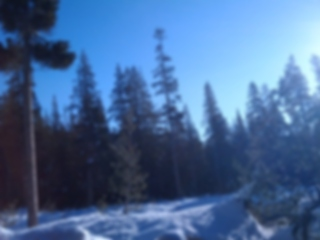
\includegraphics[width=1.5in]{figures/tahoe-blur.jpg} \\
original & blurred \\
\end{tabular}
\apiend


\apiitem{bool {\ce laplacian} (ImageBuf \&dst, const ImageBuf \&src, \\
  \bigspc\spc  ROI roi=\{\}, int nthreads=0)}
\index{ImageBufAlgo!laplacian} \indexapi{laplacian}
Return (or copy into {\cf dst}) the Laplacian of the corresponding
region of {\cf src}. The Laplacian is the generalized second derivative
of the image,
$$\frac{\partial^2 s}{\partial x^2} + \frac{\partial^2 s}{\partial y^2}$$
which is approximated by convolving the image with a discrete $3 \times 3$
Laplacian kernel,

\[ \left( \begin{array}{ccc}
0 &  1 & 0 \\
1 & -4 & 1 \\
0 &  1 & 0 \end{array} \right)\]

\smallskip
\noindent Example:
\begin{code}
    ImageBuf src ("tahoe.exr");
    ImageBuf lap = ImageBufAlgo::laplacian (src);
\end{code}

\spc \begin{tabular}{ll}
\includegraphics[width=1.5in]{figures/tahoe-small.jpg} &
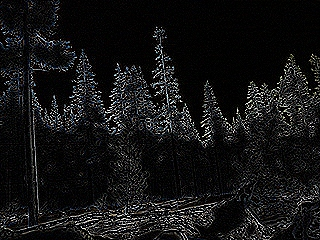
\includegraphics[width=1.5in]{figures/tahoe-laplacian.jpg} \\
original & Laplacian image \\
\end{tabular}
\apiend


\apiitem{ImageBuf {\ce fft} (const ImageBuf \&src, ROI roi=\{\}, int nthreads=0) \\
bool {\ce fft} (ImageBuf \&dst, const ImageBuf \&src, ROI roi=\{\}, int nthreads=0) \\[1.0ex]
ImageBuf {\ce ifft} (const ImageBuf \&src, ROI roi=\{\}, int nthreads=0) \\
bool {\ce ifft} (ImageBuf \&dst, const ImageBuf \&src, ROI roi=\{\}, int nthreads=0)}
\index{ImageBufAlgo!fft} \indexapi{fft}
\index{ImageBufAlgo!ifft} \indexapi{ifft}

The {\cf fft()} function takes the discrete Fourier transform (DFT) of
the section of {\cf src} denoted by {\cf roi}, returning it or storing it in {\cf dst}.
If {\cf roi} is not defined, it will be all of {\cf src}'s pixels.  Only
one channel of {\cf src} may be transformed at a time, so it will be the
first channel described by {\cf roi} (or, again, channel 0 if {\cf roi}
is undefined).  If not already in the correct format, {\cf dst} will be
re-allocated to be a 2-channel {\cf float} buffer of size
{\cf roi.width()} $\times$ {\cf roi.height}, with channel 0 being the
``real'' part and channel 1 being the the ``imaginary'' part.  The
values returned are actually the unitary DFT, meaning that it is scaled
by $1/\sqrt{\mathrm{npixels}}$.

The {\cf ifft} is the inverse discrete Fourier transform, taking a 2-channel
complex (real and imaginary) frequency domain image and transforming to a
single-channel spatial domain image.

\smallskip
\noindent Examples:
\begin{code}
    ImageBuf Src ("tahoe.exr");

    // Take the DFT of the first channel of Src
    ImageBuf Freq = ImageBufAlgo::fft (Src);

    // At this point, Freq is a 2-channel float image (real, imag)
    // Convert it back from frequency domain to a spatial image
    ImageBuf Spatial = ImageBufAlgo::ifft (Freq);
\end{code}
\apiend

\apiitem{ImageBuf {\ce complex_to_polar} (const ImageBuf \&src, ROI roi=\{\}, int nthreads=0) \\
bool {\ce complex_to_polar} (ImageBuf \&dst, const ImageBuf \&src, \\
        \bigspc\bigspc  ROI roi=\{\}, int nthreads=0) \\[1.0ex]
ImageBuf {\ce polar_to_complex} (const ImageBuf \&src, ROI roi=\{\}, int nthreads=0) \\
bool {\ce polar_to_complex} (ImageBuf \&dst, const ImageBuf \&src, \\
        \bigspc\bigspc  ROI roi=\{\}, int nthreads=0)}
\index{ImageBufAlgo!complex_to_polar} \indexapi{complex_to_polar}
\index{ImageBufAlgo!polar_to_complex} \indexapi{polar_to_complex}

The {\cf polar_to_complex()} function transforms a 2-channel image whose
channels are interpreted as complex values (real and imaginary components)
into the equivalent values expressed in polar form of amplitude and phase
(with phase between $0$ and $2\pi$).

The {\cf complex_to_polar()} function performs the reverse transformation,
converting from  polar values (amplitude and phase) to complex (real and
imaginary).

In either case,  the section of {\cf src} denoted by {\cf roi} is
transformed, storing the result in {\cf dst}. If {\cf roi} is not defined,
it will be all of {\cf src}'s pixels.  Only the first two channels of {\cf
src} will be transformed.

\smallskip
\noindent Examples:
\begin{code}
    // Suppose we have a set of frequency space values expressed as
    // amplitudes and phase...
    ImageBuf Polar ("polar.exr");

    // Convert to complex representation
    ImageBuf Complex = ImageBufAlgo::complex_to_polar (Polar);

    // Now, it's safe to take an IFFT of the complex image.
    // Convert it back from frequency domain to a spatial image.
    ImageBuf Spatial = ImageBufAlgo::ifft (Complex);
\end{code}
\apiend



\section{Image Enhancement / Restoration}
\label{sec:iba:enhance}

\apiitem{ImageBuf {\ce fixNonFinite} (const ImageBuf \&src, \\
  \bigspc\spc NonFiniteFixMode mode = NONFINITE_BOX3, \\
  \bigspc\spc int *pixelsFixed = nullptr, \\
  \bigspc\spc  ROI roi=\{\}, int nthreads=0) \\[1.0ex]
bool {\ce fixNonFinite} (ImageBuf \&dst, const ImageBuf \&src, \\
  \bigspc\spc NonFiniteFixMode mode = NONFINITE_BOX3, \\
  \bigspc\spc int *pixelsFixed = nullptr, \\
  \bigspc\spc  ROI roi=\{\}, int nthreads=0)}
\index{ImageBufAlgo!fixNonFinite} \indexapi{fixNonFinite}

Copy pixel values from {\cf src} to {\cf dst} (within the pixel and channel
range designated by {\cf roi}), and repair any non-finite ({\cf NaN} or {\cf
Inf}) pixels.  If {\cf pixelsFound} is not \NULL, store in it the number of
pixels that contained non-finite value.

How the non-finite values are repaired is specified by one of the
following modes:

\begin{description}
\item[\spc] \spc
\item[\rm \kw{NONFINITE_NONE}]   do not alter the pixels (but do count the number
                       of nonfinite pixels in {\cf *pixelsFixed}, if non-\NULL).
\item[\rm \kw{NONFINITE_BLACK}]  change non-finite values to 0.
\item[\rm \kw{NONFINITE_BOX3}]   replace non-finite values by the average of any
                     finite pixels within a 3x3 window.
\item[\rm \kw{NONFINITE_ERROR}]  do not alter non-finite values when copying,
                     but return {\cf false} and set an error if any non-finite
                     values are found.
\end{description}

This works on all pixel data types, though it's just a copy for images with
pixel data types that cannot represent {\cf NaN} or {\cf Inf} values.


\smallskip
\noindent Examples:
\begin{code}
    ImageBuf Src ("tahoe.exr");
    int pixelsFixed = 0;
    ImageBufAlgo::fixNonFinite (Src, Src, ImageBufAlgo::NONFINITE_BOX3,
                                &pixelsFixed);
    std::cout << "Repaired " << pixelsFixed << " non-finite pixels\n";
\end{code}
\apiend


\apiitem{ImageBuf {\ce fillholes_pushpull} (const ImageBuf \&src, \\
        \bigspc  ROI roi=\{\}, int nthreads=0) \\[1.0ex]
bool {\ce fillholes_pushpull} (ImageBuf \&dst, const ImageBuf \&src, \\
        \bigspc  ROI roi=\{\}, int nthreads=0)}
\index{ImageBufAlgo!fillholes_pushpull} \indexapi{fillholes_pushpull}
Copy the specified ROI of {\cf src} to {\cf dst} and fill any
holes (pixels where alpha $< 1$) with plausible values using a push-pull
technique.  The {\cf src} image must have
an alpha channel.  The dst image will end up with a copy of src, but
will have an alpha of 1.0 everywhere within {\cf roi},
and any place where the alpha
of src was < 1, dst will have a pixel color that is a plausible
``filling'' of the original alpha hole.

\smallskip
\noindent Examples:
\begin{code}
    ImageBuf Src ("holes.exr");
    ImageBuf Filled = ImageBufAlgo::fillholes_pushpull (Src);
\end{code}
\apiend


\apiitem{ImageBuf {\ce median_filter} (const ImageBuf \&src, \\
  \bigspc\spc int width = 3, int height = -1, \\
  \bigspc\spc  ROI roi=\{\}, int nthreads=0) \\[1.0ex]
bool {\ce median_filter} (ImageBuf \&dst, const ImageBuf \&src, \\
  \bigspc\spc int width = 3, int height = -1, \\
  \bigspc\spc  ROI roi=\{\}, int nthreads=0)}
\index{ImageBufAlgo!median_filter} \indexapi{median_filter}

Replace the given ROI of {\cf dst} with a median-filtered version of the
corresponding region of {\cf src}.  The median filter replaces each pixel
with the median value underneath the $\mathit{width} \times \mathit{height}$
window surrounding it. If the height is $< 1$, it will be set to width,
making a square window. The median filter tends to smooth out noise and
small high frequency details that are smaller than the window size, while
preserving the sharpness of long edges.

\smallskip
\noindent Examples:
\begin{code}
    ImageBuf Noisy ("tahoe.exr");
    ImageBuf Clean = ImageBufAlgo::median_filter (Noisy, 3, 3);
\end{code}

\spc \begin{tabular}{ccc}
\includegraphics[width=1.5in]{figures/tahoe-small.jpg} &
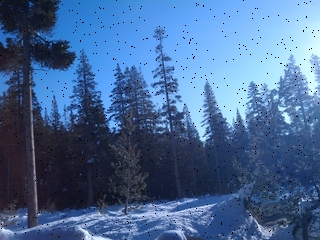
\includegraphics[width=1.5in]{figures/tahoe-pepper.jpg} &
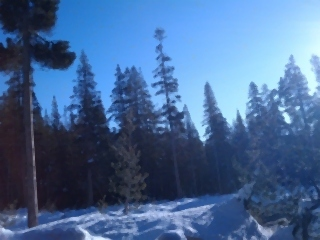
\includegraphics[width=1.5in]{figures/tahoe-pepper-median.jpg} \\
original & with dropouts & median filtered \\
\end{tabular}

\apiend


\apiitem{ImageBuf {\ce dilate} (const ImageBuf \&src, int width=3, int height=-1, \\
  \bigspc\spc  ROI roi=\{\}, int nthreads=0) \\
bool {\ce dilate} (ImageBuf \&dst, const ImageBuf \&src, int width=3, int height=-1, \\
  \bigspc\spc  ROI roi=\{\}, int nthreads=0) \\[1.0ex]
ImageBuf {\ce erode} (const ImageBuf \&src, int width=3, int height=-1, \\
  \bigspc\spc  ROI roi=\{\}, int nthreads=0) \\
bool {\ce erode} (ImageBuf \&dst, const ImageBuf \&src, int width=3, int height=-1, \\
  \bigspc\spc  ROI roi=\{\}, int nthreads=0)}
\index{ImageBufAlgo!dilate} \indexapi{dilate}
\index{ImageBufAlgo!erode} \indexapi{erode}
\index{morphological filtering}

Return (or copy into {\cf dst}) the dilated or eroded version of the
corresponding region of {\cf src}.  The dilate operation replaces each pixel
with the maximum value underneath the $\mathit{width} \times \mathit{height}$
window surrounding it, and the erode operation does the same for the minimum
value under the window. If the height is $< 1$, it will be set to width,
making a square window.

Dilation makes bright features wider and more prominent, dark features
thinner, and removes small isolated dark spots. Erosion makes dark features
wider, bright features thinner, and removes small isolated bright spots.

Dilation and erosion are basic morphological filters, and more complex ones
are often constructed from them:
\begin{itemize}
\item
\item ``open'' is erode followed by dilate, and it keeps the overall shape
while removing small bright regions;
\item ``close'' is dilate followed by erode, and it keeps the overall shape
while removing small dark regions;
\item ``morphological gradient'' is dilate minus erode, which gives a
bright perimeter edge;
\item ``tophat'' is the original source minus the ``open'', which isolates
local peaks;
\item ``bottomhat'' is the ``close'' minus the original source, which
isolates dark holes.
\end{itemize}

\smallskip
\noindent Examples:
\begin{code}
    ImageBuf Source ("source.tif");

    ImageBuf Dilated = ImageBufAlgo::dilate (Source, 3, 3);
    ImageBuf Eroded  = ImageBufAlgo::erode (Source, 3, 3);

    // Morphological "open" is dilate(erode((source))
    ImageBuf Opened = ImageBufAlgo::dilate (Eroded, 3, 3);
    // Morphological "close" is erode(dilate(source))
    ImageBuf Closed = ImageBufAlgo::erode (Dilated, 3, 3);
    // Morphological "gradient" is dilate minus erode
    ImageBuf Gradient = ImageBufAlgo::sub (Dilated, Eroded);
    // Tophat filter is source minus open
    ImageBuf Tophad = ImageBufAlgo::sub (Source, Opened);
    // Bottomhat filter is close minus source
    ImageBuf Bottomhat = ImageBufAlgo::sub (Close, Source);
\end{code}

\begin{tabular}{cccc}

\includegraphics[width=1.0in]{figures/morphsource.jpg} &

\includegraphics[width=1.0in]{figures/dilate.jpg} &

\includegraphics[width=1.0in]{figures/erode.jpg} &

\includegraphics[width=1.0in]{figures/morphopen.jpg} \\
original & dilate & erode & open \\[2.0ex]

\includegraphics[width=1.0in]{figures/morphclose.jpg} &

\includegraphics[width=1.0in]{figures/morphgradient.jpg} &
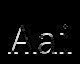
\includegraphics[width=1.0in]{figures/tophat.jpg} &
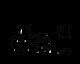
\includegraphics[width=1.0in]{figures/bottomhat.jpg} \\
close & gradient & tophat & bottomhat \\
\end{tabular}

\apiend


\apiitem{ImageBuf {\ce unsharp_mask} (const ImageBuf \&src, \\
  \bigspc\spc string_view kernel = "gaussian", float width = 3.0f, \\
  \bigspc\spc float contrast = 1.0f, float threshold = 0.0f, \\
  \bigspc\spc  ROI roi=\{\}, int nthreads=0) \\[1.0ex]
bool {\ce unsharp_mask} (ImageBuf \&dst, const ImageBuf \&src, \\
  \bigspc\spc string_view kernel = "gaussian", float width = 3.0f, \\
  \bigspc\spc float contrast = 1.0f, float threshold = 0.0f, \\
  \bigspc\spc  ROI roi=\{\}, int nthreads=0)}
\index{ImageBufAlgo!unsharp_mask} \indexapi{unsharp_mask}
\label{sec:iba:unsharpmask}

Return (or copy into {\cf dst}) a sharpened version of the
corresponding region of {\cf src} using the ``unsharp mask'' technique.
Unsharp masking basically works by first blurring the image (low
pass filter), subtracting this from the original image, then
adding the residual back to the original to emphasize the edges.
Roughly speaking,

\begin{code}
     dst = src + contrast * thresh(src - blur(src))
\end{code}

The specific blur can be selected by kernel name and width (for example,
\qkw{gaussian} is typical). As a special case, \qkw{median} is also accepted
as the kernel name, in which case a median filter is performed rather than
a blurring convolution (Gaussian and other blurs sometimes over-sharpen edges,
whereas using the median filter will sharpen compact high-frequency details
while not over-sharpening long edges).

The {\cf contrast} is a multiplier on the overall sharpening effect.  The
thresholding step causes all differences less than {\cf threshold} to be
squashed to zero, which can be useful for suppressing sharpening of
low-contrast details (like noise) but allow sharpening of
higher-contrast edges.

\smallskip
\noindent Examples:
\begin{code}
    ImageBuf Blurry ("tahoe.exr");
    ImageBuf Sharp = ImageBufAlgo::unsharp_mask (Blurry, "gaussian", 5.0f);
\end{code}
\apiend


\section{Color manipulation}
\label{sec:iba:color}

\apiitem{ImageBuf {\ce colorconvert} (const ImageBuf \&src, \\
  \bigspc\spc string_view from, string_view to, bool unpremult=true, \\
  \bigspc\spc string_view context_key="", string_view context_value="", \\
  \bigspc\spc ColorConfig *colorconfig=nullptr, \\
  \bigspc\spc ROI roi=\{\}, int nthreads=0) \\
bool {\ce colorconvert} (ImageBuf \&dst, const ImageBuf \&src, \\
  \bigspc\spc string_view from, string_view to, bool unpremult=true, \\
  \bigspc\spc string_view context_key="", string_view context_value="", \\
  \bigspc\spc ColorConfig *colorconfig=nullptr, \\
  \bigspc\spc ROI roi=\{\}, int nthreads=0) \\[1.0ex]
ImageBuf {\ce colorconvert} (const ImageBuf \&src, \\
  \bigspc\spc const ColorProcessor *processor, bool unpremult=true, \\
  \bigspc\spc  ROI roi=\{\}, int nthreads=0) \\
bool {\ce colorconvert} (ImageBuf \&dst, const ImageBuf \&src, \\
  \bigspc\spc const ColorProcessor *processor, bool unpremult=true, \\
  \bigspc\spc  ROI roi=\{\}, int nthreads=0)}
\index{ImageBufAlgo!colorconvert} \indexapi{colorconvert}
Return (or copy into {\cf dst}) the pixels of {\cf src} within the ROI,
applying a color transform to the pixel values.

If {\cf unpremult} is {\cf true} and the image has an alpha channel,
unpremultiply (divide color channels by alpha) before color conversion, then
premultiply again after the color conversion.

The first form of this function specifies the ``from'' and ``to'' color
spaces by name. An optional {\cf ColorConfig} is specified, but {\cf nullptr}
is passed, the default OCIO color configuration found by examining the {\cf
\$OCIO} environment variable will be used instead.

The second form is directly passed a {\cf ColorProcessor}, which is is a
special object created by a {\cf ColorConfig} (see {\cf OpenImageIO/color.h}
for details).

The {\cf context_key} and {\cf context_value} may optionally be used
to establish a context (for example, a shot-specific transform).

If OIIO was built with OpenColorIO support enabled, then the transformation
may be between any two spaces supported by the active OCIO configuration, or
may be a ``look'' transformation created by {\cf
ColorConfig::createLookTransform}.  If OIIO was not built with OpenColorIO
support enabled, then the only transformations available are from \qkw{sRGB}
to \qkw{linear} and vice versa.

\smallskip
\noindent Examples:
\begin{code}
    #include <OpenImageIO/imagebufalgo.h>
    #include <OpenImageIO/color.h>
    using namespace OIIO;

    ImageBuf Src ("tahoe.jpg");
    ColorConfig cc;
    ColorProcessor *processor = cc.createColorProcessor ("vd8", "lnf");
    ImageBuf dst = ImageBufAlgo::colorconvert (Src, processor, true);
    ColorProcessor::deleteColorProcessor (processor);

    // Equivalent, though possibly less efficient if you will be
    // converting many images using the same transformation:
    ImageBuf Src ("tahoe.jpg");
    ImageBuf Dst = ImageBufAlgo::colorconvert (Src, "vd8", "lnf", true);
\end{code}
\apiend

\apiitem{ImageBuf {\ce ociolook} (const ImageBuf \&src, \\
  \bigspc\spc string_view looks, string_view from, string_view to, \\
  \bigspc\spc bool inverse=false, bool unpremult=true, \\
  \bigspc\spc string_view context_key="", string_view context_value="", \\
  \bigspc\spc ColorConfig *colorconfig=NULL, \\
  \bigspc\spc ROI roi=\{\}, int nthreads=0) \\[1.0ex]
bool {\ce ociolook} (ImageBuf \&dst, const ImageBuf \&src, \\
  \bigspc\spc string_view looks, string_view from, string_view to, \\
  \bigspc\spc bool inverse=false, bool unpremult=true, \\
  \bigspc\spc string_view context_key="", string_view context_value="", \\
  \bigspc\spc ColorConfig *colorconfig=NULL, \\
  \bigspc\spc ROI roi=\{\}, int nthreads=0)}
\index{ImageBufAlgo!ociolook} \indexapi{ociolook}
Return (or copy into {\cf dst}) the pixels of {\cf src} within the ROI,
applying an OpenColorIO ``look'' transform to the pixel values.
The {\cf context_key} and {\cf context_value} may optionally be used
to establish a context (for example, a shot-specific transform).

If {\cf inverse} is {\cf true}, it will reverse the color transformation
and look application.

If {\cf unpremult} is {\cf true} and the image has an alpha channel,
unpremultiply (divide color channels by alpha) before color conversion, then
premultiply again after the color conversion.

An optional {\cf ColorConfig} is specified, but {\cf NULL} is passed, the
default OCIO color configuration found by examining the {\cf \$OCIO}
environment variable will be used instead.

\smallskip
\noindent Examples:
\begin{code}
    ImageBuf Src ("tahoe.jpg");
    ImageBuf Dst = ImageBufAlgo::ociolook (Src, "look", "vd8", "lnf",
                                           true, false, "SHOT", "pe0012");
\end{code}
\apiend


\apiitem{ImageBuf {\ce ociodisplay} (const ImageBuf \&src, string_view display,\\
  \bigspc\spc string_view view, string_view from="", string_view looks="",\\
  \bigspc\spc bool unpremult=true, string_view key="", string_view value="", \\
  \bigspc\spc ColorConfig *colorconfig=nullptr, \\
  \bigspc\spc ROI roi=\{\}, int nthreads=0) \\[1.0ex]
bool {\ce ociodisplay} (ImageBuf \&dst, const ImageBuf \&src, string_view display,\\
  \bigspc\spc string_view view, string_view from="", string_view looks="",\\
  \bigspc\spc bool unpremult=true, string_view key="", string_view value="", \\
  \bigspc\spc ColorConfig *colorconfig=nullptr, \\
  \bigspc\spc ROI roi=\{\}, int nthreads=0)}
\index{ImageBufAlgo!ociodisplay} \indexapi{ociodisplay}
Return (or copy into {\cf dst}) the pixels of {\cf src} within the ROI,
applying an OpenColorIO ``display'' transform to the pixel values.
If {\cf from} or {\cf looks} are empty, it will not
override the look or source color space (subtly different than
passing \qkw{}, the empty string, which means to use no look or source
space).  The {\cf key} and {\cf value} may optionally be used
to establish a context (for example, a shot-specific transform).

If {\cf inverse} is {\cf true}, it will reverse the color transformation
and look application.

If {\cf unpremult} is {\cf true} and the image has an alpha channel,
unpremultiply (divide color channels by alpha) before color conversion, then
premultiply again after the color conversion.

An optional {\cf ColorConfig} is specified, but {\cf nullptr} is passed, the
default OCIO color configuration found by examining the {\cf \$OCIO}
environment variable will be used instead.

\smallskip
\noindent Examples:
\begin{code}
    ImageBuf Src ("tahoe.exr");
    ImageBuf Dst = ImageBufAlgo::ociodisplay (Src, "sRGB", "Film", "lnf",
                                              "", true, "SHOT", "pe0012");
\end{code}
\apiend


\apiitem{ImageBuf {\ce ociofiletransform} (const ImageBuf \&src, \\
  \bigspc\spc string_view name, bool inverse=false, bool unpremult=true, \\
  \bigspc\spc ColorConfig *colorconfig=nullptr, \\
  \bigspc\spc ROI roi=\{\}, int nthreads=0) \\[1.0ex]
bool {\ce ociofiletransform} (ImageBuf \&dst, const ImageBuf \&src, \\
  \bigspc\spc string_view name, bool inverse=false, bool unpremult=true, \\
  \bigspc\spc ColorConfig *colorconfig=nullptr, \\
  \bigspc\spc ROI roi=\{\}, int nthreads=0)}
\index{ImageBufAlgo!ociofiletransform} \indexapi{ociofiletransform}
Return (or copy into {\cf dst}) the pixels of {\cf src} within the ROI,
applying an OpenColorIO ``file'' transform to the pixel values. If {\cf inverse} is {\cf
true}, it will reverse the color transformation and look application.

If {\cf unpremult} is {\cf true} and the image has an alpha channel,
unpremultiply (divide color channels by alpha) before color conversion, then
premultiply again after the color conversion.

An optional {\cf ColorConfig} is specified, but {\cf nullptr} is passed, the
default OCIO color configuration found by examining the {\cf \$OCIO}
environment variable will be used instead.

\smallskip
\noindent Examples:
\begin{code}
    ImageBuf Src ("tahoe.jpg");
    ImageBuf Dst = ImageBufAlgo::ociofiletransform (Src, "footransform.csp");
\end{code}
\apiend


\apiitem{ImageBuf {\ce unpremult} (const ImageBuf \&src, ROI roi=\{\}, int nthreads=0)\\
bool {\ce unpremult} (ImageBuf \&dst, const ImageBuf \&src, ROI roi=\{\}, int nthreads=0) \\[1.0ex]
ImageBuf {\ce premult} (const ImageBuf \&src, ROI roi=\{\}, int nthreads=0) \\
bool {\ce premult} (ImageBuf \&dst, const ImageBuf \&src, ROI roi=\{\}, int nthreads=0)}
\index{ImageBufAlgo!unpremult} \indexapi{unpremult}

The {\cf unpremult} operation returns (or copies into dst) the pixels of src within the ROI, and in the process
divides all color channels (those not alpha or z)
by the alpha value, to ``un-premultiply'' them.  This presumes that the
image starts of as ``associated alpha'' a.k.a.\ ``premultipled.''

The {\cf premult} operation returns (or copies into dst) the pixels of src within the ROI, and in the process
multiplies all color channels (those not alpha or z)
by the alpha value, to ``premultiply'' them.  This presumes that the
image starts of as ``unassociated alpha'' a.k.a.\ ``non-premultipled.''

Both operations are simply a copy if there is no identified alpha channel
(and a no-op if {\cf dst} and {\cf src} are the same image).

\smallskip
\noindent Examples:
\begin{code}
    // Convert in-place from associated alpha to unassociated alpha
    ImageBuf A ("a.exr");
    ImageBufAlgo::unpremult (A, A);

    // Convert in-place from unassociated alpha to associated alpha
    ImageBufAlgo::premult (A, A);
\end{code}
\apiend



\section{Import / export}
\label{sec:iba:importexport}

\apiitem{bool {\ce make_texture} (MakeTextureMode mode, const ImageBuf \&input, \\
\bigspc                             string_view outputfilename,
                             const ImageSpec \&config,\\
\bigspc                             std::ostream *outstream = nullptr) \\
bool {\ce make_texture} (MakeTextureMode mode, string_view filename, \\
\bigspc                             string_view outputfilename,
                             const ImageSpec \&config,\\
\bigspc                             std::ostream *outstream = nullptr)}
\index{ImageBufAlgo!make_texture} \indexapi{make_texture}

Turn an image file (either an existing \ImageBuf or specified by {\cf
filename}) into a tiled, MIP-mapped, texture file and write to the
file named by ({\cf outputfilename}).  The {\cf mode} describes what type of texture file we
are creating and may be one of the following:

\noindent \begin{tabular}{p{2in}p{3.1in}}
{\cf MakeTxTexture} & Ordinary 2D texture\\
%MakeTxShadow & \\
{\cf MakeTxEnvLatl} & Latitude-longitude environment map\\
{\cf \small MakeTxEnvLatlFromLightProbe} & Latitude-longitude environment map
       constructed from a ``light probe'' image.\\
{\cf MakeTxBumpWithSlopes} & Bump/displacement map with extra slope
    data channels (6 channels total, containing both the height and 1st and
    2nd moments of slope distributions) for bump-to-roughness conversion in
    shaders. \\
\end{tabular}

If the {\cf outstream} pointer is not \NULL, it should point
to a stream (for example, {\cf \&std::out}, or a pointer to a local 
{\cf std::stringstream} to capture output), which is where console output
and error messages will be deposited.

The {\cf config} is an \ImageSpec that contains all the information and
special instructions for making the texture.  Anything set in {\cf config}
(format, tile size, or named metadata) will take precedence over
whatever is specified by the input file itself.  Additionally, named
metadata that starts with \qkw{maketx:} will not be output to the file
itself, but may contain instructions controlling how the texture is
created.  The full list of supported configuration options is:

\noindent Named fields:

\begin{tabular}{ >{\cf}l p{4in}}
   format         & Data format of the texture file (default: UNKNOWN =
                    same format as the input) \\
   tile_width     & \multirow{3}{*}{Preferred tile size (default: 64x64x1)} \\
   tile_height    &       \\
   tile_depth     & \\
\end{tabular}
\medskip

\noindent Metadata in {\cf config.extra_attribs}:

\begin{longtable}{ >{\spc \cf\small}p{1.8in} >{\cf\small}l p{3in}}
   compression & string &   Default: "zip" \\
   fovcot & float &          Default: aspect ratio of the image resolution \\
   planarconfig & string &  Default: "separate" \\
   worldtocamera & matrix &  World-to-camera matrix of the view. \\
   worldtoscreen & matrix &  World-to-screen space matrix of the view. \\
   wrapmodes & string &     Default: "black,black" \\
   maketx:verbose & int &    How much detail should go to outstream (0). \\
   maketx:stats & int &      If nonzero, print stats to outstream (0). \\
   maketx:resize & int &     If nonzero, resize to power of 2. (0) \\
   maketx:nomipmap & int &   If nonzero, only output the top MIP level (0). \\
   maketx:updatemode & int &  If nonzero, write new output only if the
                             output file doesn't already exist, or is
                             older than the input file, or was created with
                             different command-line arguments. (0) \\
   \multicolumn{2}{l}{\spc \cf\small maketx:constant_color_detect} \\  & int &
                          If nonzero, detect images that are entirely
                            one color, and change them to be low
                            resolution (default: 0). \\
   \multicolumn{2}{l}{\spc \cf\small maketx:monochrome_detect} \\ & int &
                          If nonzero, change RGB images which have
                             R==G==B everywhere to single-channel
                             grayscale (default: 0). \\
   maketx:opaque_detect & int &
                          If nonzero, drop the alpha channel if alpha
                             is 1.0 in all pixels (default: 0). \\
   maketx:unpremult & int &  If nonzero, unpremultiply color by alpha before
                             color conversion, then multiply by alpha
                             after color conversion (default: 0). \\
   {\small maketx:incolorspace} & string & \\
   {\small maketx:outcolorspace} & string &
                          These two together will apply a color conversion
                              (with OpenColorIO, if compiled). Default: \qkw{} \\
   {\small maketx:colorconfig} & string &
                          Specifies a custom OpenColorIO color config file.
                              Default: \qkw{} \\
   maketx:checknan & int &   If nonzero, will consider it an error if the
                              input image has any NaN pixels. (0) \\
   maketx:fixnan & string & If set to "black" or "box3", will attempt
                              to repair any NaN pixels found in the
                              input image (default: "none"). \\
   \multicolumn{2}{l}{\spc \cf\small maketx:set_full_to_pixels} \\ & int &
                          If nonzero, doctors the full/display window
                              of the texture to be identical to the
                              pixel/data window and reset the origin
                              to 0,0 (default: 0). \\
   maketx:filtername & string &
                          If set, will specify the name of a high-quality
                             filter to use when resampling for MIPmap
                             levels. Default: \qkw{}, use bilinear resampling. \\
   maketx:highlightcomp & int &
                          If nonzero, performs highlight compensation --
                             range compression and expansion around 
                             the resize, plus clamping negative plxel
                             values to zero. This reduces ringing when
                             using filters with negative lobes. \\
   maketx:nchannels & int &  If nonzero, will specify how many channels
                             the output texture should have, padding with
                             0 values or dropping channels, if it doesn't
                             the number of channels in the input.
                             (default: 0, meaning keep all input channels) \\
   maketx:channelnames & string &
                          If set, overrides the channel names of the
                             output image (comma-separated). \\
   {\small maketx:fileformatname} & string &
                          If set, will specify the output file format.
                              (default: \qkw{}, meaning infer the format from
                              the output filename) \\
   \multicolumn{2}{l}{\spc \cf\small maketx:prman_metadata} \\ & int &
                          If set, output some metadata that PRMan will
                              need for its textures. (0) \\
   {\small maketx:oiio_options} & int &
                          (Deprecated; all are handled by default) \\
   \multicolumn{2}{l}{\spc \cf\small maketx:prman_options} \\ & int &
                          If nonzero, override a whole bunch of settings 
                              as needed to make textures that are
                              compatible with PRMan. (0) \\
   maketx:mipimages & string &
                          Semicolon-separated list of alternate images
                              to be used for individual MIPmap levels,
                              rather than simply downsizing. (default: \qkw{}) \\
   \multicolumn{2}{l}{\spc \cf\small maketx:full_command_line} \\ & string &
                          The command or program used to generate this
                              call, will be embedded in the metadata.
                              (default: \qkw{}) \\
   \multicolumn{2}{l}{\spc \cf\small maketx:ignore_unassoc} \\ & int &
                          If nonzero, will disbelieve any evidence that
                              the input image is unassociated alpha. (0) \\
   \multicolumn{2}{l}{\spc \cf\small maketx:read_local_MB} \\ & int &
                          If nonzero, will read the full input file locally
                              if it is smaller than this threshold. Zero
                              causes the system to make a good guess at
                                a reasonable threshold (e.g. 1 GB). (0) \\
   maketx:forcefloat & int &
                          Forces a conversion through float data for
                              the sake of ImageBuf math. (1) \\
   maketx:hash & int &
                          Compute the sha1 hash of the file in parallel. (1) \\
   \multicolumn{2}{l}{\spc \cf\small maketx:allow_pixel_shift} \\ & int &
                          Allow up to a half pixel shift per mipmap level.
                              The fastest path may result in a slight shift
                              in the image, accumulated for each mip level
                              with an odd resolution. (0) \\
\end{longtable}

\smallskip
\noindent Examples:
\begin{code}
    // This command line:
    //    maketx in.exr --hicomp --filter lanczos3 --opaque-detect \
    //             -o texture.exr
    // is equivalent to:

    ImageBuf Input ("in.exr");
    ImageSpec config;
    config.attribute ("maketx:highlightcomp", 1);
    config.attribute ("maketx:filtername", "lanczos3");
    config.attribute ("maketx:opaquedetect", 1);
    stringstream s;
    bool ok = ImageBufAlgo::make_texture (ImageBufAlgo::MakeTxTexture,
                                          Input, "texture.exr", config, &s);
    if (! ok)
        std::cout << "make_texture error: " << s.str() << "\n";
\end{code}
\apiend


\apiitem{ImageBuf {\ce from_IplImage} (const IplImage *ipl, TypeDesc convert=TypeUnknown)}
\index{ImageBufAlgo!from_IplImage} \indexapi{from_IplImage}
\index{OpenCV}\indexapi{IplImage}\index{Intel Image Library}
Convert an {\cf IplImage}, used by OpenCV and Intel's Image Libray, to
an \ImageBuf (copying the pixels).  If {\cf convert} is
not set to {\cf UNKNOWN}, try to establish the result as holding that
data type and convert the {\cf IplImage} data.  Return {\cf true} if ok,
{\cf false} if it couldn't figure out how to make the conversion from
{\cf IplImage} to an \ImageBuf.  If OpenImageIO was compiled without OpenCV
support, this function will fail.

\begin{comment}
\smallskip
\noindent Examples:
\begin{code}
\end{code}
\end{comment}
\apiend


\apiitem{IplImage* {\ce to_IplImage} (const ImageBuf \&src)}
\index{ImageBufAlgo!to_IplImage} \indexapi{to_IplImage}
\index{OpenCV}\indexapi{IplImage}\index{Intel Image Library}
Construct an {\cf IplImage*}, used by OpenCV and Intel's Image Library,
that is equivalent to the \ImageBuf {\cf src}.  If it is not possible, or
if OpenImageIO was compiled without OpenCV support, then return
{\cf nullptr}.  The ownership of the {\cf IplImage} is fully transferred to the
calling application.

\begin{comment}
\smallskip
\noindent Examples:
\begin{code}
\end{code}
\end{comment}
\apiend


\apiitem{ImageBuf {\ce capture_image} (int cameranum, TypeDesc convert=TypeUnknown)}
\index{ImageBufAlgo!capture_image} \indexapi{capture_image}
Capture a still image from a designated camera.  If able to do so,
store the image in {\cf dst} and return {\cf true}.  If there is no such device,
or support for camera capture is not available (such as if OpenCV
support was not enabled at compile time), return {\cf false} and do not
alter {\cf dst}.

\smallskip
\noindent Examples:
\begin{code}
    ImageBuf WebcamImage = ImageBufAlgo::capture_image (0, TypeDesc::UINT8);
    WebcamImage.save ("webcam.jpg");
\end{code}
\apiend



\section{Deep images}
\label{sec:iba:deep}

A number of {\cf ImageBufAlgo} functions are designed to work with ``deep''
images. These are detailed below. In general, {\cf ImageBufAlgo} functions
not listed in this section should not be expected to work with deep images.

\subsection{Functions specific to deep images}

\apiitem{ImageBuf {\ce deepen} (const ImageBuf \&src, float zvalue, \\
        \bigspc  ROI roi=\{\}, int nthreads=0) \\[1.0ex]
bool {\ce deepen} (ImageBuf \&dst, const ImageBuf \&src, float zvalue, \\
        \bigspc  ROI roi=\{\}, int nthreads=0)}
\index{ImageBufAlgo!deepen} \indexapi{deepen} \index{deep images}
Return (or copy into {\cf dst}) pixels from regular (not ``deep'') image {\cf src}.
Turning a flat image image into a deep one means:

If the {\cf src} image has a \qkw{Z} channel: if the source pixel's {\cf Z}
channel value is not infinite, the corresponding pixel of {\cf dst} will get
a single depth sample that copies the data from the soruce pixel; otherwise,
{\cf dst} will get an empty pixel. In other words, infinitely far pixels
will not turn into deep samples.

If the {\cf src} image lacks a \qkw{Z} channel: if any of the source pixel's
channel values are nonzero, the corresponding pixel of {\cf dst} will get a
single depth sample that copies the data from the source pixel and uses the
{\cf zvalue} parameter for the depth; otherwise, if all source channels in
that pixel are zero, the destination pixel will get no depth samples.

If {\cf src} is already a deep image, it will just copy pixel values from
{\cf src}.

\smallskip
\noindent Examples:
\begin{code}
    ImageBuf Flat ("RGBAZ.exr");
    ImageBuf Deep = ImageBufAlgo::deepen (Flat);
\end{code}
\apiend

\apiitem{ImageBuf {\ce flatten} (const ImageBuf \&src, ROI roi=\{\}, int nthreads=0) \\[1.0ex]
bool {\ce flatten} (ImageBuf \&dst, const ImageBuf \&src, ROI roi=\{\}, int nthreads=0)}
\index{ImageBufAlgo!flatten} \indexapi{flatten} \index{deep images}
Return (or copy into {\cf dst}) the ``flattened'' composite of deep image
{\cf src}. That is, it converts a deep image to a simple flat image by
compositing the depth samples within each pixel to yield a single ``flat''
value per pixel. If {\cf src} is not deep, it just copies the pixels without
alteration.

\smallskip
\noindent Examples:
\begin{code}
    ImageBuf Deep ("deepalpha.exr");
    ImageBuf Flat = ImageBufAlgo::flatten (Deep);
\end{code}
\apiend

\apiitem{ImageBuf {\ce deep_merge} (const ImageBuf \&A, const ImageBuf \&B, \\
        \bigspc\spc bool occlusion_cull=true, ROI roi=\{\}, int nthreads=0) \\[1.0ex]
bool {\ce deep_merge} (ImageBuf \&dst, const ImageBuf \&A, const ImageBuf \&B, \\
        \bigspc\spc bool occlusion_cull=true, ROI roi=\{\}, int nthreads=0)}
\index{ImageBufAlgo!deep_merge} \indexapi{deep_merge} \index{deep images}
Merge the samples of two \emph{deep} images {\cf A} and {\cf B} into deep
result {\cf dst}. If {\cf occlusion_cull} is {\cf true}, samples beyond
the first opaque sample will be discarded, otherwise they will be kept.

\smallskip
\noindent Examples:
\begin{code}
    ImageBuf DeepA ("hardsurf.exr");
    ImageBuf DeepB ("volume.exr");
    ImageBuf Merged = ImageBufAlgo::deep_merge (DeepA, DeepB);
\end{code}
\apiend

\apiitem{ImageBuf {\ce deep_holdout} (const ImageBuf \&src, const ImageBuf \&holdout, \\
\bigspc\spc  ROI roi=\{\}, int nthreads=0)\\[1.0ex]
bool {\ce deep_holdout} (ImageBuf \&dst, const ImageBuf \&src, \\
\bigspc\spc  const ImageBuf \&holdout, ROI roi=\{\}, int nthreads=0)}
\index{ImageBufAlgo!deep_holdout} \indexapi{deep_holdout} \index{deep images}

Merge the deep pixels of two images, using {\cf holdout} as a deep holdout
mask against {\cf src}.

\smallskip
\noindent Examples:
\begin{code}
    ImageBuf Src ("image.exr");
    ImageBuf Holdout ("holdout.exr");
    ImageBuf Merged = ImageBufAlgo::deep_holdout (Src, Holdout);
\end{code}
\apiend


\subsection{General functions that also work for deep images}

\apiitem{ImageBuf {\ce channels} (const ImageBuf \&src, int nchannels, \\
        \bigspc  cspan<int> channelorder,  cspan<float> channelvalues=NULL, \\
        \bigspc                 cspan<std::string> newchannelnames=\{\}, \\
        \bigspc                 bool shuffle_channel_names=false) \\
bool {\ce channels} (ImageBuf \&dst, const ImageBuf \&src, int nchannels, \\
        \bigspc  cspan<int> channelorder,  cspan<float> channelvalues=NULL, \\
        \bigspc                 cspan<std::string> newchannelnames=\{\}, \\
        \bigspc                 bool shuffle_channel_names=false)}
Reorder, rename, remove, or add channels to a deep image.
See Section~\ref{sec:iba:channels}
\apiend

\apiitem{bool {\ce compare} (const ImageBuf \&A, const ImageBuf \&B, \\
  \bigspc float failthresh, float warnthresh, CompareResults \&result,\\
   \bigspc  ROI roi=\{\}, int nthreads=0)}
Numerically compare two images.
\apiend

\apiitem{bool {\ce computePixelStats} (PixelStats \&stats, const ImageBuf \&src, \\
   \bigspc\bigspc  ROI roi=\{\}, int nthreads=0)}
Compute per-channel statistics about the image.
See Section~\ref{sec:iba:computePixelStats}
\apiend

\apiitem{ImageBuf {\ce crop} (const ImageBuf \&src, ROI roi=\{\}, int nthreads=0) \\
bool {\ce crop} (ImageBuf \&dst, const ImageBuf \&src, ROI roi=\{\}, int nthreads=0)}
\index{ImageBufAlgo!crop} \indexapi{crop}
Crop the specified region of {\cf src}, discarding samples outside the ROI.
\apiend

\apiitem{ROI {\ce nonzero_region} (const ImageBuf \&src, ROI roi=\{\}, int nthreads=0)}
\index{ImageBufAlgo!nonzero_region} \indexapi{nonzero_region}
For ``deep'' images, this function returns the smallest ROI that contains
all pixels that contain depth samples, and excludes the border pixels
that contain no depth samples at all.
\apiend

\apiitem{ImageBuf {\ce add} (const ImageBuf \&A, cspan<float> B, ROI roi=\{\}, int nthreads=0) \\
bool {\ce add} (ImageBuf \&dst, const ImageBuf \&A, cspan<float> B, \\
        \bigspc ROI roi=\{\}, int nthreads=0) \\
ImageBuf {\ce sub} (const ImageBuf \&A, cspan<float> B, ROI roi=\{\}, int nthreads=0) \\
bool {\ce sub} (ImageBuf \&dst, const ImageBuf \&A, cspan<float> B, \\
        \bigspc ROI roi=\{\}, int nthreads=0) \\[1.0ex]
ImageBuf {\ce mul} (const ImageBuf \&A, cspan<float> B, ROI roi=\{\}, int nthreads=0) \\
bool {\ce mul} (ImageBuf \&dst, const ImageBuf \&A, cspan<float> B, \\
        \bigspc ROI roi=\{\}, int nthreads=0) \\
ImageBuf {\ce div} (const ImageBuf \&A, cspan<float> B, ROI roi=\{\}, int nthreads=0) \\
bool {\ce div} (ImageBuf \&dst, const ImageBuf \&A, cspan<float> B, \\
        \bigspc ROI roi=\{\}, int nthreads=0)}
\index{ImageBufAlgo!add} \indexapi{add}
\index{ImageBufAlgo!sub} \indexapi{sub}
\index{ImageBufAlgo!mul} \indexapi{mul}
\index{ImageBufAlgo!div} \indexapi{div}

Add, subtract, multiply, or divide all the samples in a deep image {\cf A}
by per-channel values {\cf B[]}.
\apiend

\apiitem{ImageBuf {\ce fixNonFinite} (const ImageBuf \&src, \\
  \bigspc\spc NonFiniteFixMode mode = NONFINITE_BOX3, \\
  \bigspc\spc int *pixelsFixed = nullptr, ROI roi=\{\}, int nthreads=0) \\
bool {\ce fixNonFinite} (ImageBuf \&dst, const ImageBuf \&src, \\
  \bigspc\spc NonFiniteFixMode mode = NONFINITE_BOX3, \\
  \bigspc\spc int *pixelsFixed = nullptr, ROI roi=\{\}, int nthreads=0)}
\index{ImageBufAlgo!fixNonFinite} \indexapi{fixNonFinite}
Repair nonfinite ({\cf NaN} or {\cf Inf}) values, setting them to 0.0.
\apiend

\apiitem{ImageBuf {\ce resample} (const ImageBuf \&src, bool interpolate = true, \\
        \bigspc ROI roi=\{\}, int nthreads=0) \\[1.0ex]
bool {\ce resample} (ImageBuf \&dst, const ImageBuf \&src, bool interpolate = true, \\
        \bigspc ROI roi=\{\}, int nthreads=0)}
\index{ImageBufAlgo!resample} \indexapi{resample}
Compute a resized version of the
corresponding portion of {\cf src} (mapping such that the ``full'' image
window of each correspond to each other, regardless of resolution), for each
pixel merely copying the closest deep pixel of the source image (no true
interpolation is done for deep images).
\apiend


\begin{comment}
\apiitem{bool {\ce blah} (ImageBuf \&dst, const ImageBuf \&src, \\
        \bigspc  ROI roi=ROI::All(), int nthreads=0)}
\index{ImageBufAlgo!blah} \indexapi{blah}
Blah.
\smallskip
\noindent Examples:
\begin{code}
\end{code}
\apiend
\end{comment}

\index{ImageBufAlgo|)}
\index{Image Processing|)}

\chapwidthend
